\section{Frontend}

All'interno di questa sezione verrà descritto il modulo \textit{Frontend}, il quale si occupa di gestire l'interfaccia grafica dell'applicazione richiedendo le informazioni necessarie al modulo \textit{Backend} e creando richieste agli smart contracts visti nel capitolo \hyperref[sec:blockchain-module]{\textit{Blockchain}}.
Il framework utilizzato per lo sviluppo è \textit{React}, il quale permette di creare applicazioni web responsive e dinamiche. In aggiunta, è stato deciso di utilizzare il linguaggio \textit{TypeScript} per lo sviluppo del modulo, in quanto permette di definire tipi statici per le variabili e di conseguenza di ridurre gli errori di programmazione.

\subsection{Librerie}

Per il corretto funzionamento del modulo sono state scelte alcune librerie di fondamentale importanza. Di seguito verranno elencate e descritte le principali.

\begin{itemize}
    \item \textit{WalletConnect}\footnote{https://walletconnect.com/}: libreria che permette di connettersi ad un wallet di diverso tipo (Web extension, Mobile, Desktop) e di conseguenza di interagire con la blockchain.
    \item \textit{Wagmi}\footnote{https://wagmi.sh/}: Consigliata da \textit{WalletConnect} per compatibilità, permette di creare transazioni e ottenere informazioni in Ethereum.
    \item \textit{ChakraUI}\footnote{https://chakra-ui.com/}: libreria grafica semplice e con una vasta gamma di componenti.
    \item \textit{React Router}\footnote{https://reactrouter.com/}: libreria che permette di gestire il routing all'interno di un'applicazione React. Con possibilità di creare una
    \textit{Single Page Application}.
\end{itemize}

\subsection{Struttura}
\label{sec:frontend-structure}

Sebbene React stesso non consigli una struttura file specifica \cite{react-structure}, è fondamentale organizzare il codice in modo da rendere la lettura e la manutenzione più semplice. Perciò, è stato deciso di dividere il codice seguendo questo schema:

\begin{lstlisting}[basicstyle=\small]
    src/
        assets/
            Imagini
        components/
            Ogni componente in una cartella separata
        pages/
            Ogni pagina in una cartella separata
        hooks/
            Hooks personalizzati
        context/
            Context providers
        utils/
            Funzioni di utility, ognuna in una cartella separata
        styles/
            Stile globale
        services/
            Servizi di comunicazione con il backend e blockchain
\end{lstlisting}

Inoltre, internamente alle cartelle \textit{assets}, \textit{components}, \textit{pages}, i file sono organizzati nel seguente modo:

\begin{lstlisting}[basicstyle=\small]
    NFTCard/
        __mocks__/
            NFTCard.tsx
        __tests__/
            __snapshots__/ # autogenerato
                NFTCard.test.tsx.snap 
          NFTCard.tsx
          useNFTCard.tsx
        NFTCard.tsx
        useNFTCard.tsx
\end{lstlisting}

L'esempio soprastante mostra la struttura del componente \textit{NFTCard}. All'interno della sua cartella sono presenti i file \textit{NFTCard.tsx} e \textit{useNFTCard.tsx}, i quali contengono rispettivamente il componente grafico ed il suo hook personalizzato. Questo approccio permette un ottimo livello di \textit{Separation of Concerns} e di conseguenza una maggiore manutenibilità del codice. Proseguendo, all'interno della cartella \textit{\_\_tests\_\_} sono presenti i file di test per il componente e per il suo \textit{hook}. Nel caso in cui sia necessario effettuare dei test sulla parte grafica, \textit{jest} genera automaticamente uno \textit{snapshot} del componente, il quale viene utilizzato per verificare che non ci siano cambiamenti involontari. Infine, all'interno della cartella \textit{\_\_mocks\_\_} è presente il file \textit{NFTCard.tsx} che viene utilizzato per simulare il componente durante i test in altri componenti.

\subsection{Componenti ricorrenti}

Nella cartella \textit{components} sono presenti i componenti che vengono utilizzati più volte all'interno delle pagine dell'applicazione. Di seguito una breve descrizione di ciascun componente.

\begin{itemize}
    \item \textit{PageLayout}: Gestisce il layout della pagina includendo l'header e il footer.
    \item \textit{AccountPopover}: Mostra le possibili azioni che l'utente può effettuare sul proprio account.
    \item \textit{NFTHistoryTable}: Mostra la cronologia delle transazioni effettuate sull'NFT.
    \item \textit{NFTCard}: Card per la visualizzazione di un NFT.
    \item \textit{NFTCardGrid}: Griglia di NFTCard.
    \item \textit{CollectionGrid}: Griglia di NFTCard organizzate per collezione.
    \item \textit{NFTORCollectionViewer}: Permette il cambio di visualizzazione tra NFTCardGrid e CollectionGrid.
    \item \textit{Buy}: Bottone per l'acquisto di un NFT comprensivo di modale per la conferma dell'acquisto.
    \item \textit{ModifySale}: Bottone per la modifica di un NFT in vendita comprensivo di modale per la conferma della modifica.
    \item \textit{CancelSale}: Bottone per la rimozione di un NFT dalla vendita comprensivo di modale per la conferma della rimozione.
    \item \textit{Sell}: Bottone per la messa in vendita di un NFT comprensivo di modale per la conferma della messa in vendita.
    \item \textit{NFTOperations}: Permette di visualizzare i bottoni di Buy, ModifySale, CancelSale, Sell in base allo stato dell'NFT e all'utente connesso.
    \item \textit{PriceDisibution}: Fornisce una visualizzazione grafica della distribuzione del prezzo di vendita di un NFT.
    \item \textit{Error}: Mostra un messaggio di errore.
    \item \textit{LoadingButton}: Bottone con un indicatore di caricamento.
    \item \textit{LoadingSpinner}: Indicatore di caricamento.
    \item \textit{ShadowButton}: Bottone standard dell'applicazione.
    \item \textit{UploadImage}: Gestisce il caricamento, cancellazione e visualizzazione di un'immagine.
    \item \textit{WithdrawRoyaltyButton}: Bottone per il ritiro delle royalty.
\end{itemize}

\subsection{Pagine}
Nel seguente capitolo verranno visualizzate e descritte le pagine dell'applicazione. Ogni pagina presenta la possibilità di cambiare tema tra \textit{light} e \textit{dark} ed è completamente \textit{responsive}, adattandosi a qualsiasi dispositivo. Essendo l'applicativo sviluppato dinamico e reattivo saranno discusse unicamente le pagine in fase iniziale e non quelle in seguito a delle azioni dell'utente. Inoltre, per ogni pagina verrà mostrata la versione desktop e mobile.

\subsubsection{Home}

La pagina \textit{Home} è la prima pagina che viene visualizzata all'apertura del sito. Il suo scopo è quello di mostrare gli NFT che sono attualmente in vendita. Nel caso in cui il wallet non sia collegato sarà visualizzato un messaggio che invita l'utente a collegarlo, altrimenti apparirà come in figura \ref{fig:home}.

\begin{figure}[H]
    \begin{minipage}{0.7\textwidth}
      \centering
      \fcolorbox{mint-cream}{white}{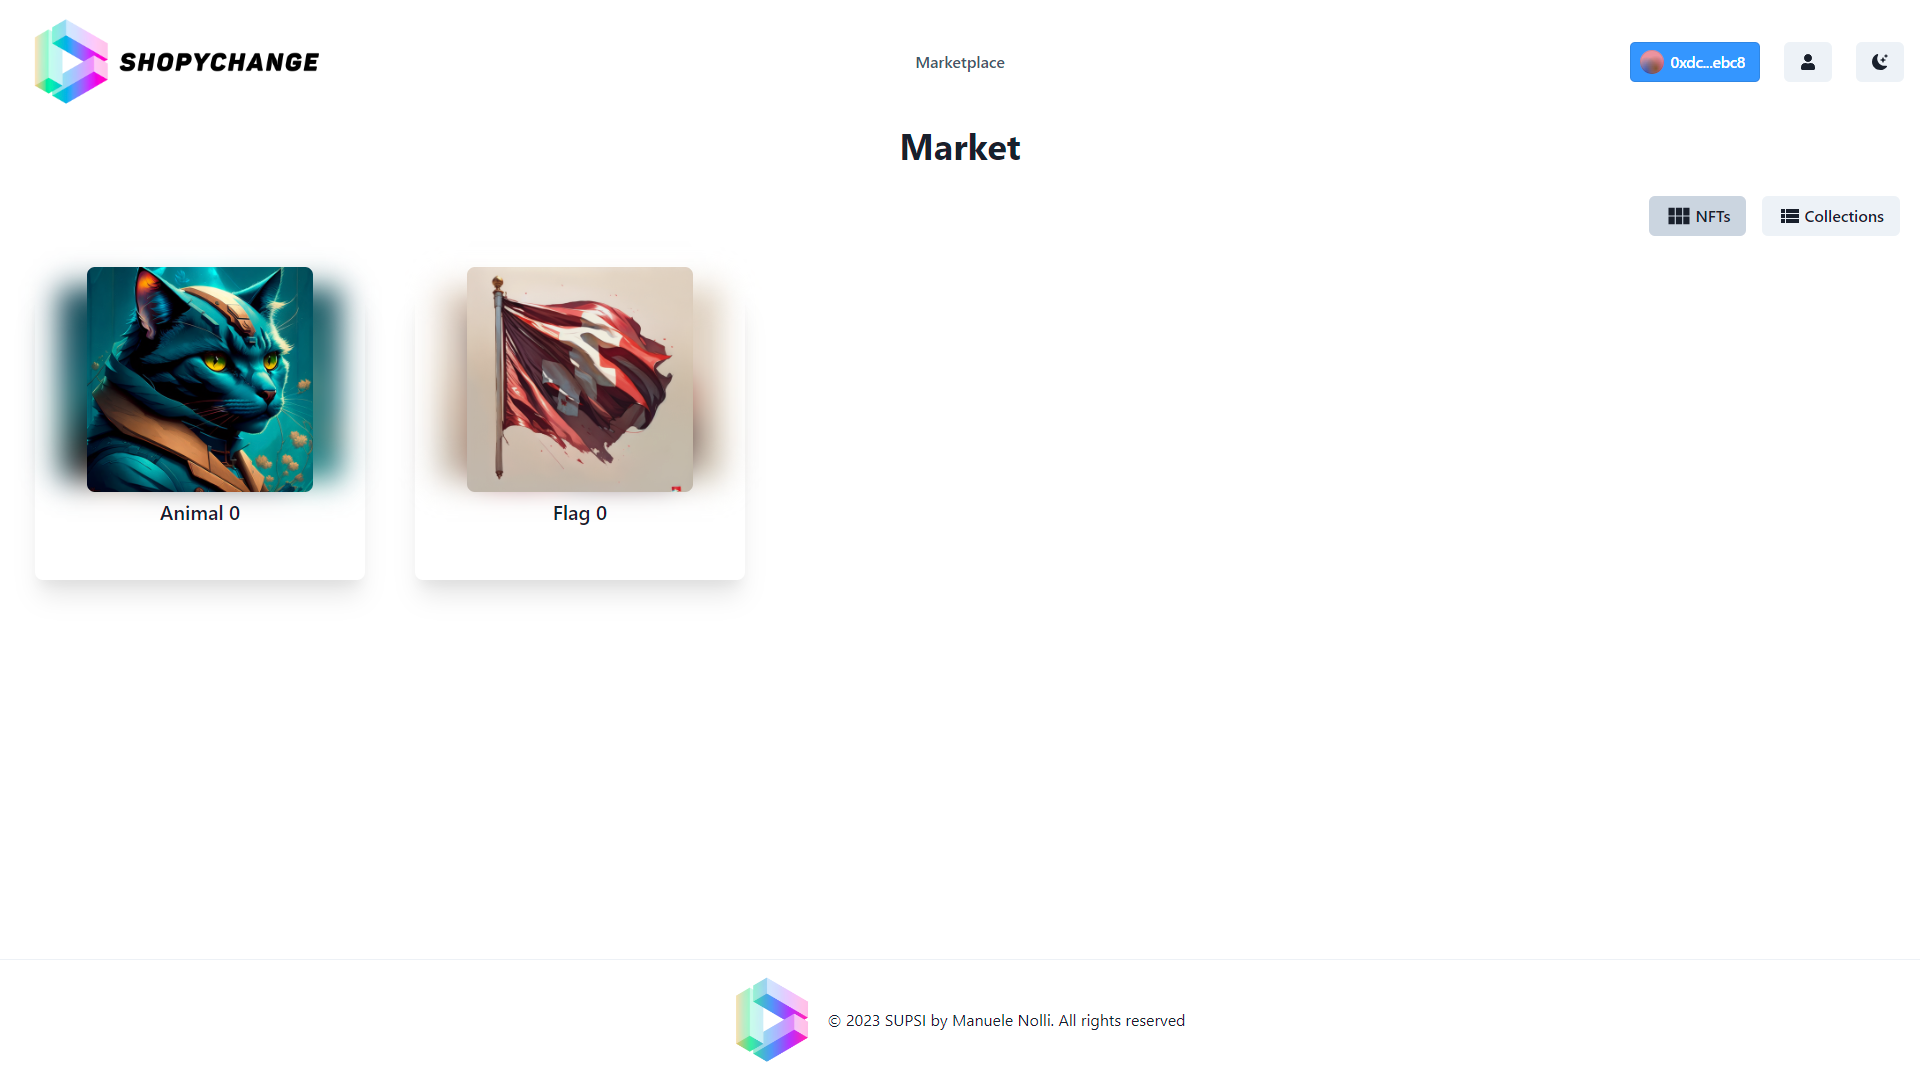
\includegraphics[width=\textwidth]{images/pages/home_connected.png}}
    \end{minipage}
    \hfill
    \begin{minipage}{0.26\textwidth }
      \centering
      \fcolorbox{mint-cream}{white}{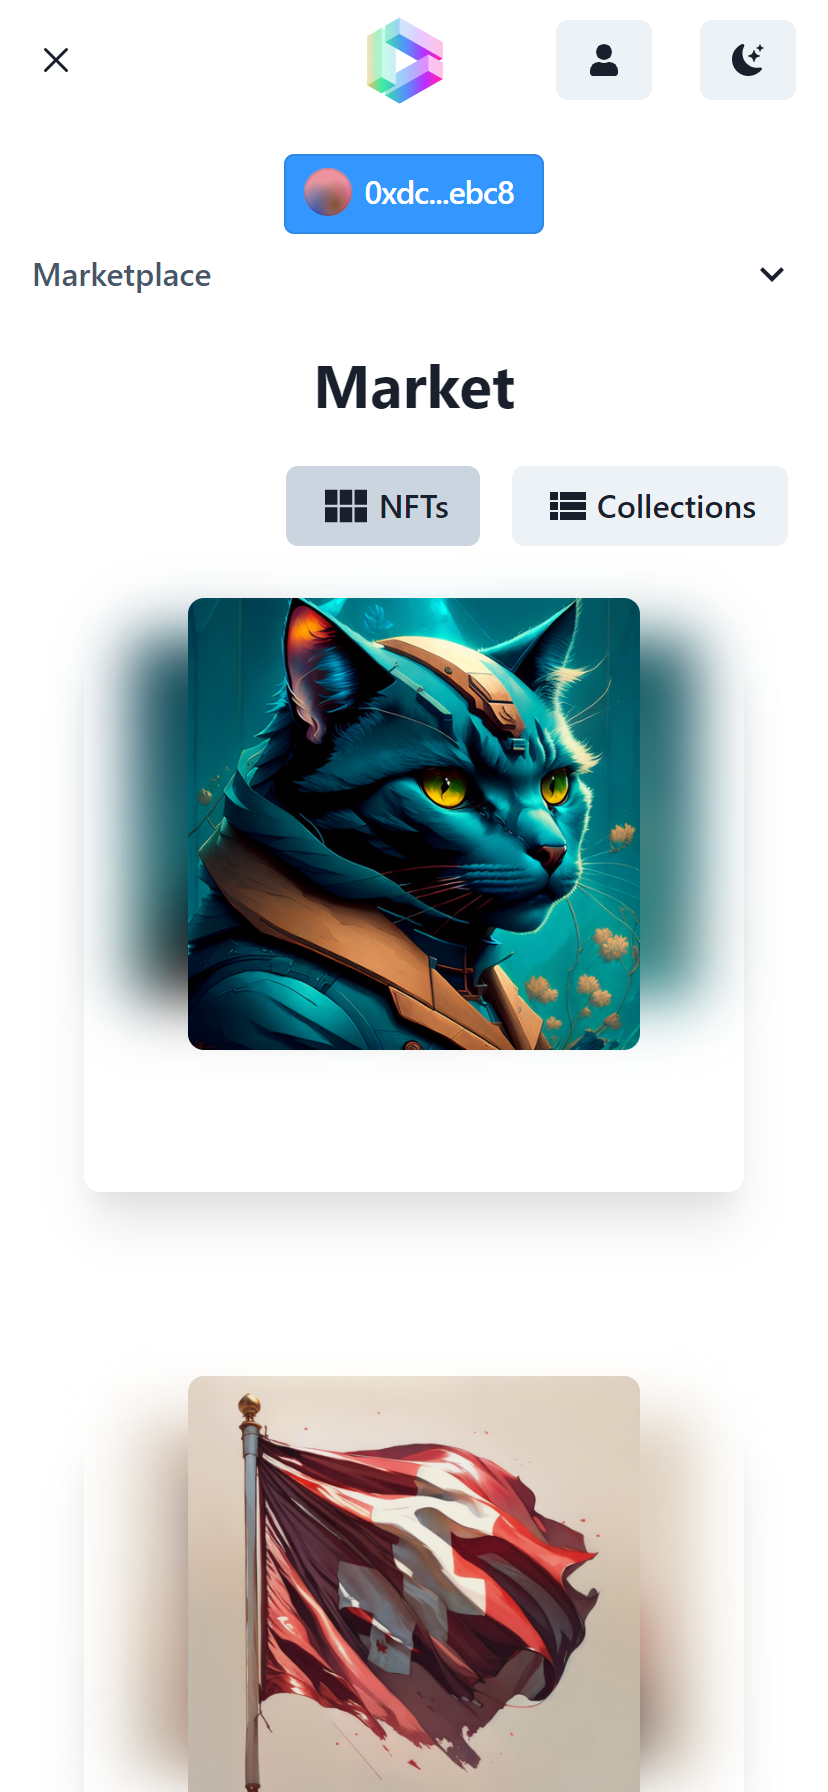
\includegraphics[width=\textwidth]{images/pages/home_connected_mobile.png}}
      \end{minipage}
      \caption{Pagina Home}
      \label{fig:home}
  \end{figure}
  
\subsubsection{Account}

All'interno della pagine \textit{Account} è possibile vedere gli NFT posseduti. In aggiunta, in questa pagina è possibile, tramite la sidebar, navigare alla pagina di aggiunta di collezioni osservate. Inoltre, all'interno della sidebar è presente anche la voce \textit{Favorite NFTs}, la quale purtroppo non è stata implementata per mancanza di tempo. La pagina è visibile in figura \ref{fig:account}.

\begin{figure}[H]
    \begin{minipage}{0.7\textwidth}
      \centering
      \fcolorbox{mint-cream}{white}{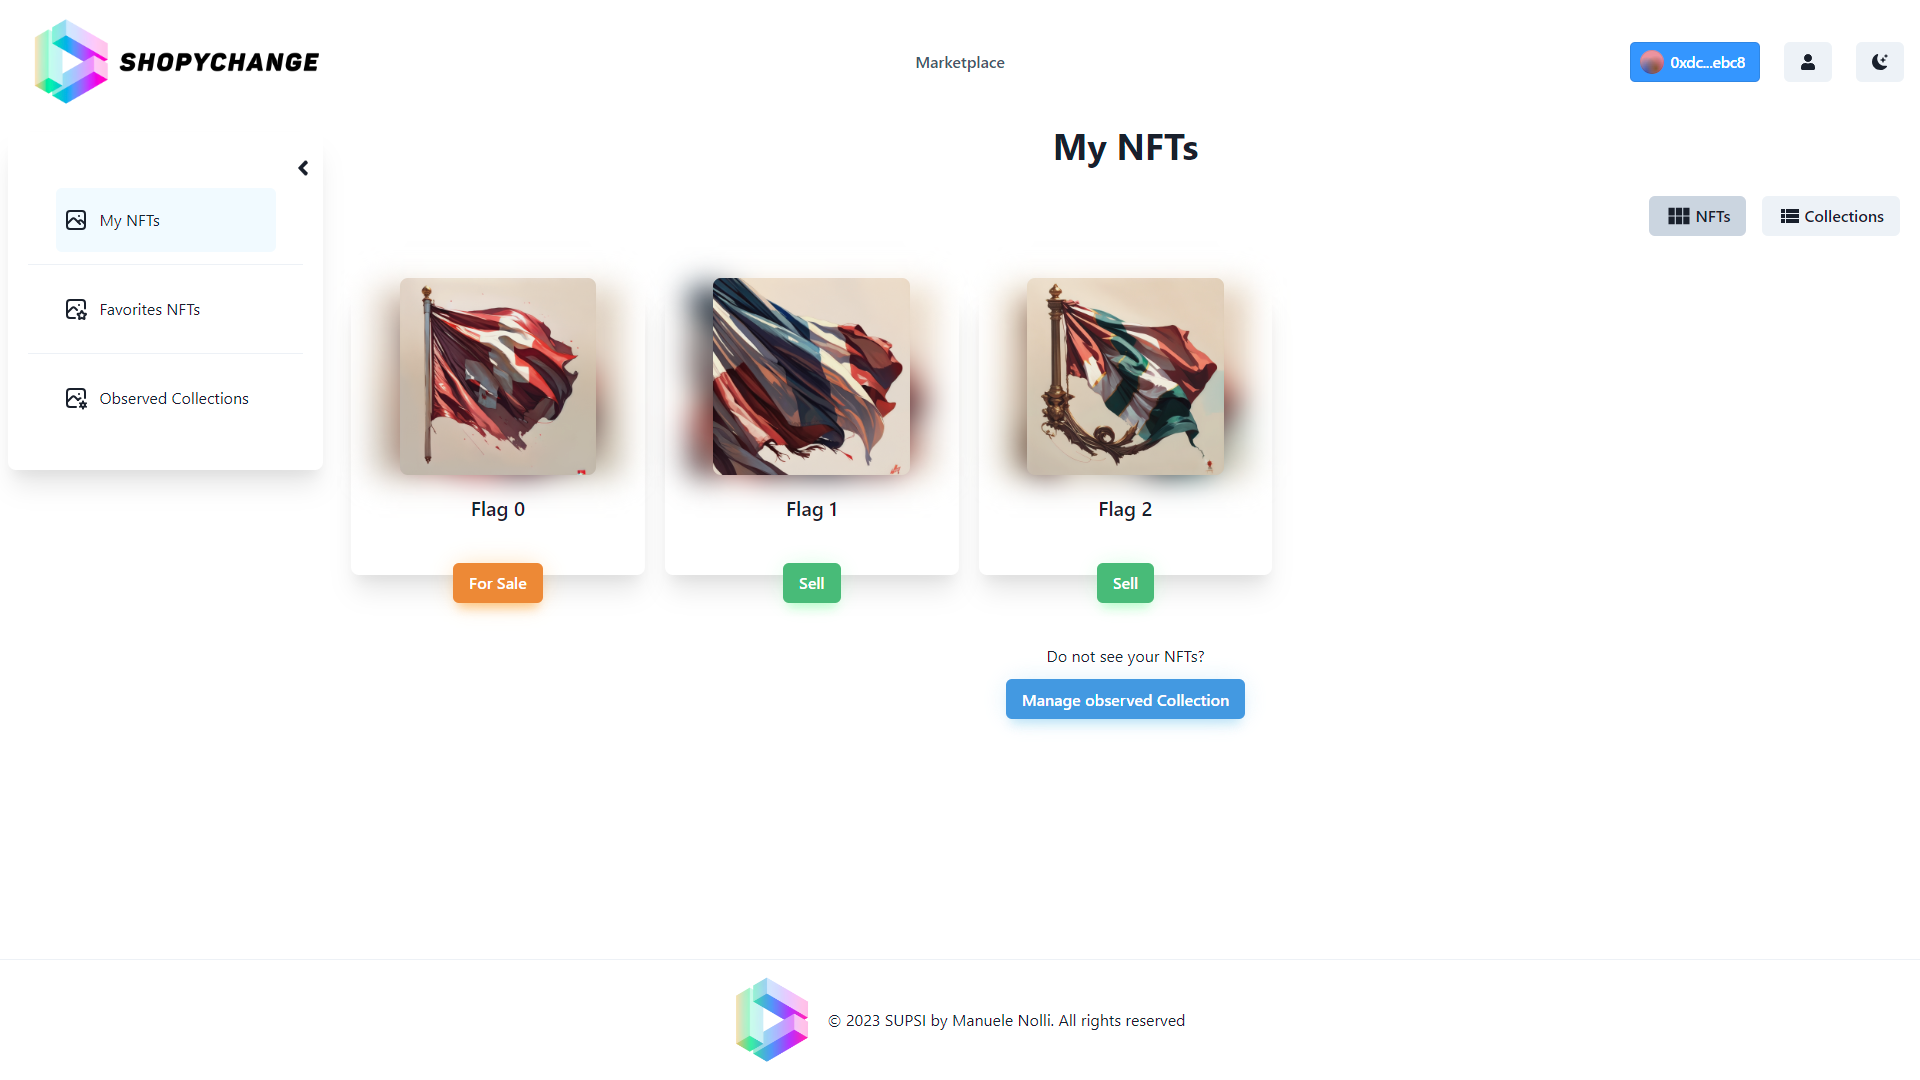
\includegraphics[width=\textwidth]{images/pages/myNFT.png}}
    \end{minipage}
    \hfill
    \begin{minipage}{0.26\textwidth }
      \centering
      \fcolorbox{mint-cream}{white}{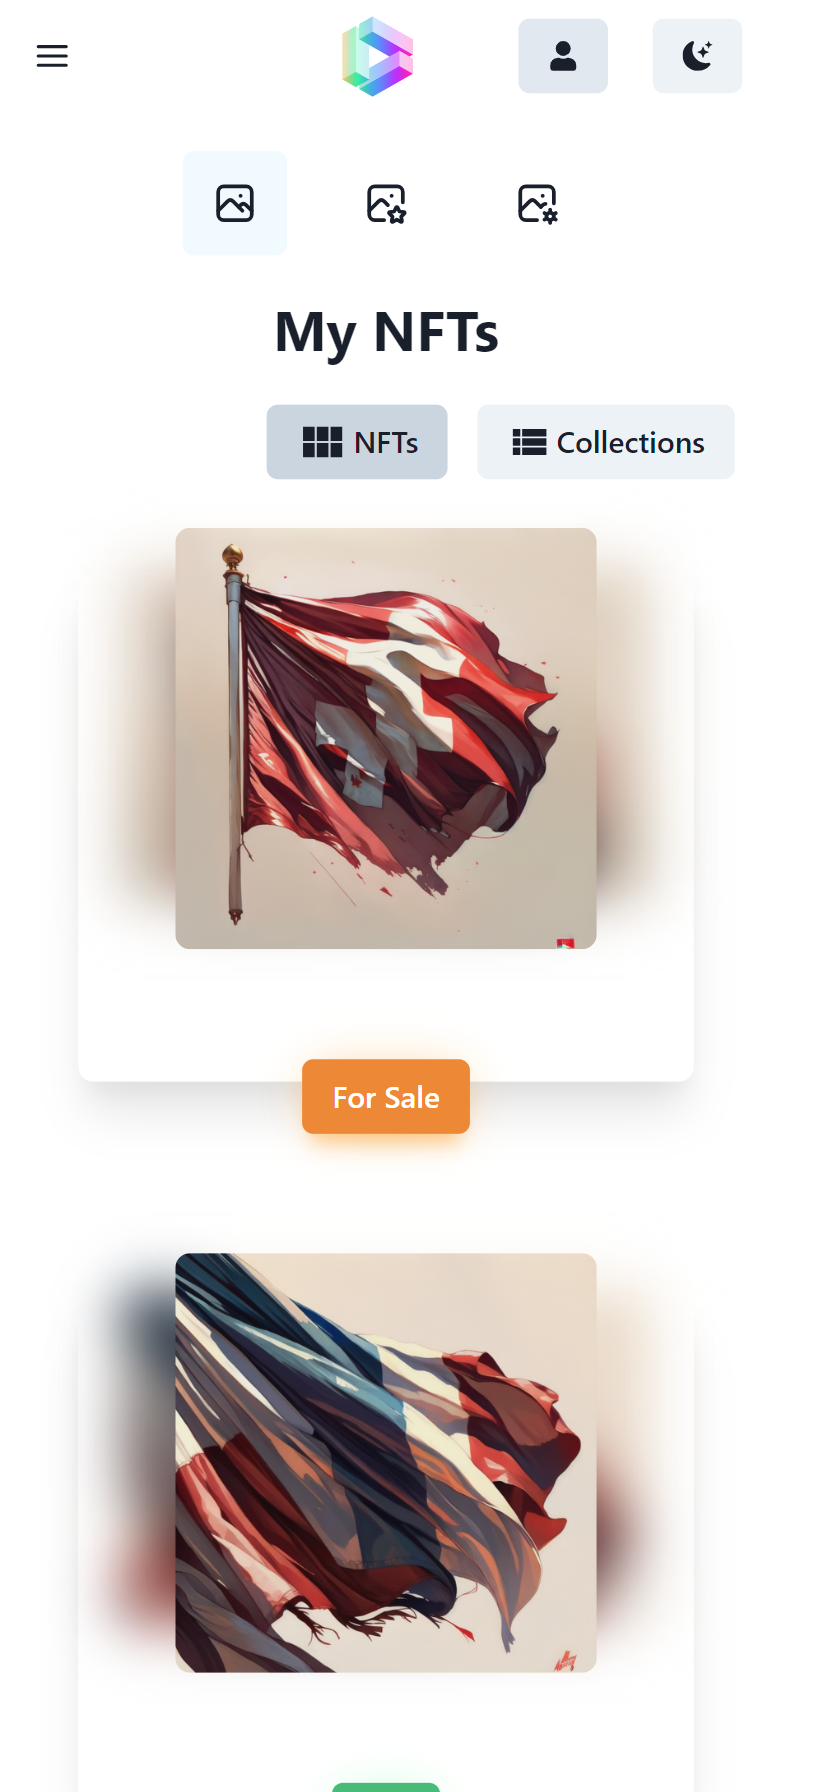
\includegraphics[width=\textwidth]{images/pages/myNFT_mobile.png}}
      \end{minipage}
      \caption{Pagina Account}
      \label{fig:account}
  \end{figure}

\subsubsection{Creazione}
\label{sec:creazione}

La pagina \textit{Creazione} è raggiungibile tramite il pulsante Account nell'header, il suo scopo è tramite due grandi pulsanti di direzionare l'utente alla pagina di creazione di un NFT o di una collezione. Le due pagine sono visibili nelle figure \ref{fig:create-nft} e \ref{fig:create-collection}. Entrambe contengono un form per l'inserimento dei dati e la possibilità di caricare una o più immagini. Il form è completamente validato e non permette l'invio di dati errati. 

\begin{figure}[H]
    \begin{minipage}{0.7\textwidth}
      \centering
      \fcolorbox{mint-cream}{white}{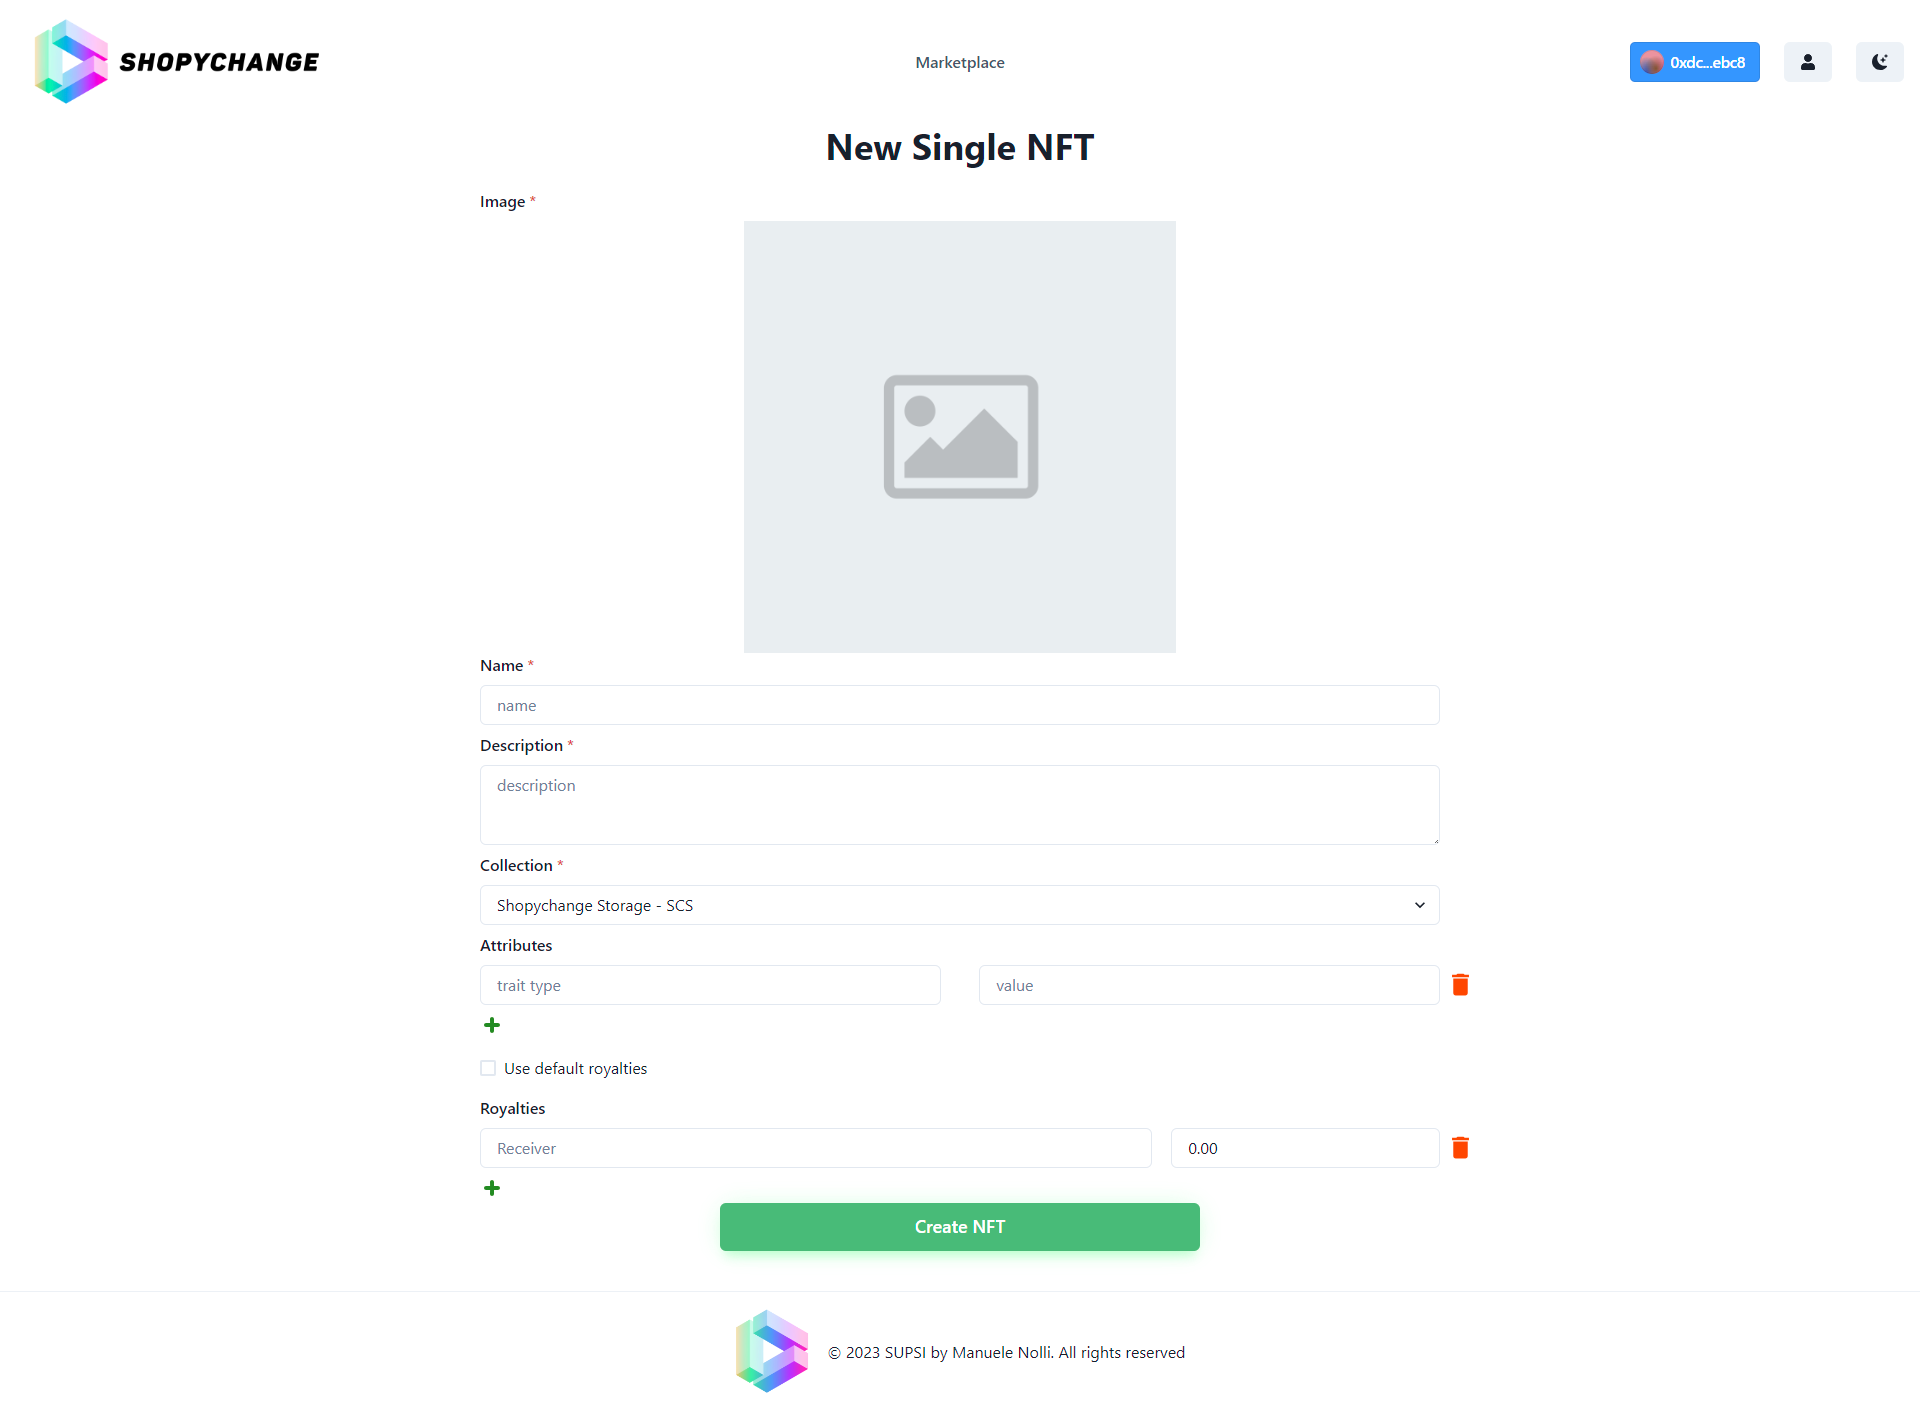
\includegraphics[width=\textwidth]{images/pages/createNFT.png}}
    \end{minipage}
    \hfill
    \begin{minipage}{0.26\textwidth }
      \centering
      \fcolorbox{mint-cream}{white}{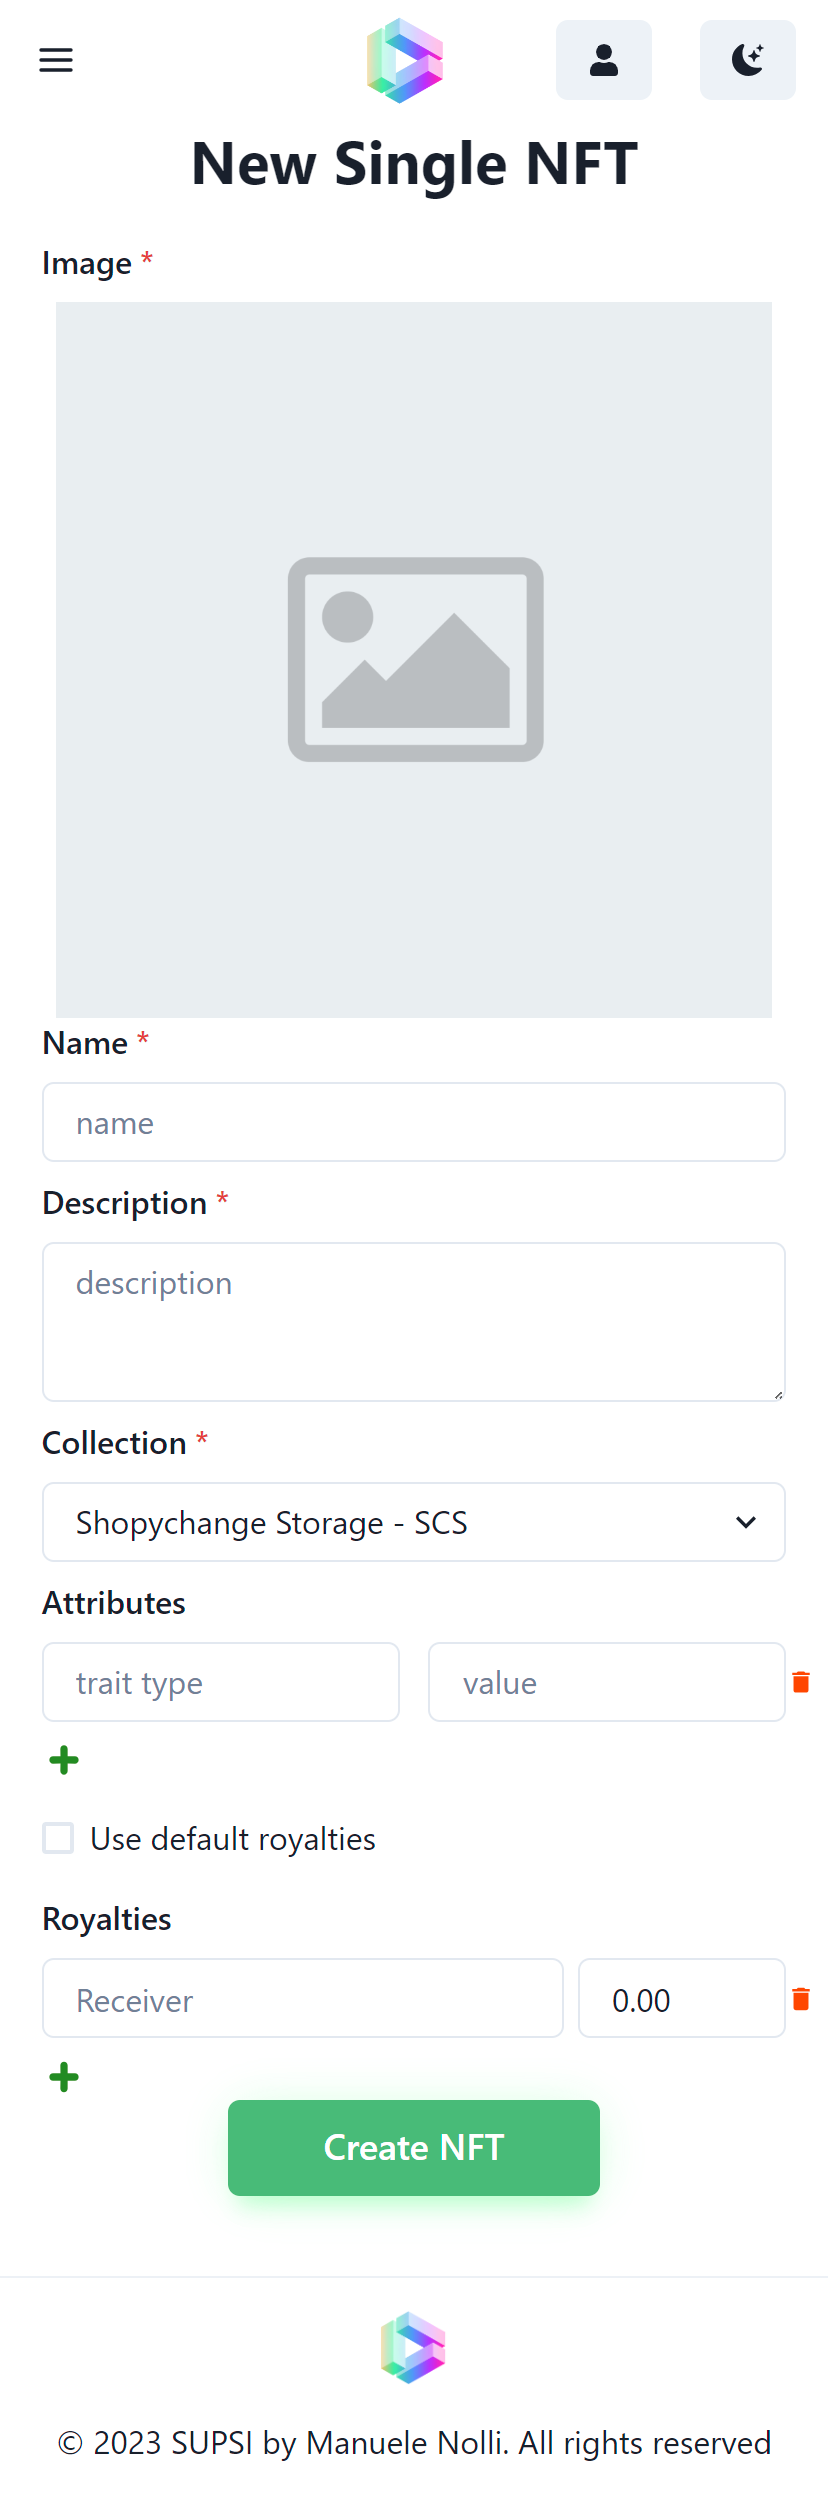
\includegraphics[width=\textwidth]{images/pages/createNFT_mobile.png}}
      \end{minipage}
      \caption{Pagina Creazione NFT}
      \label{fig:create-nft}
  \end{figure}

\begin{figure}[H]
    \begin{minipage}{0.7\textwidth}
      \centering
      \fcolorbox{mint-cream}{white}{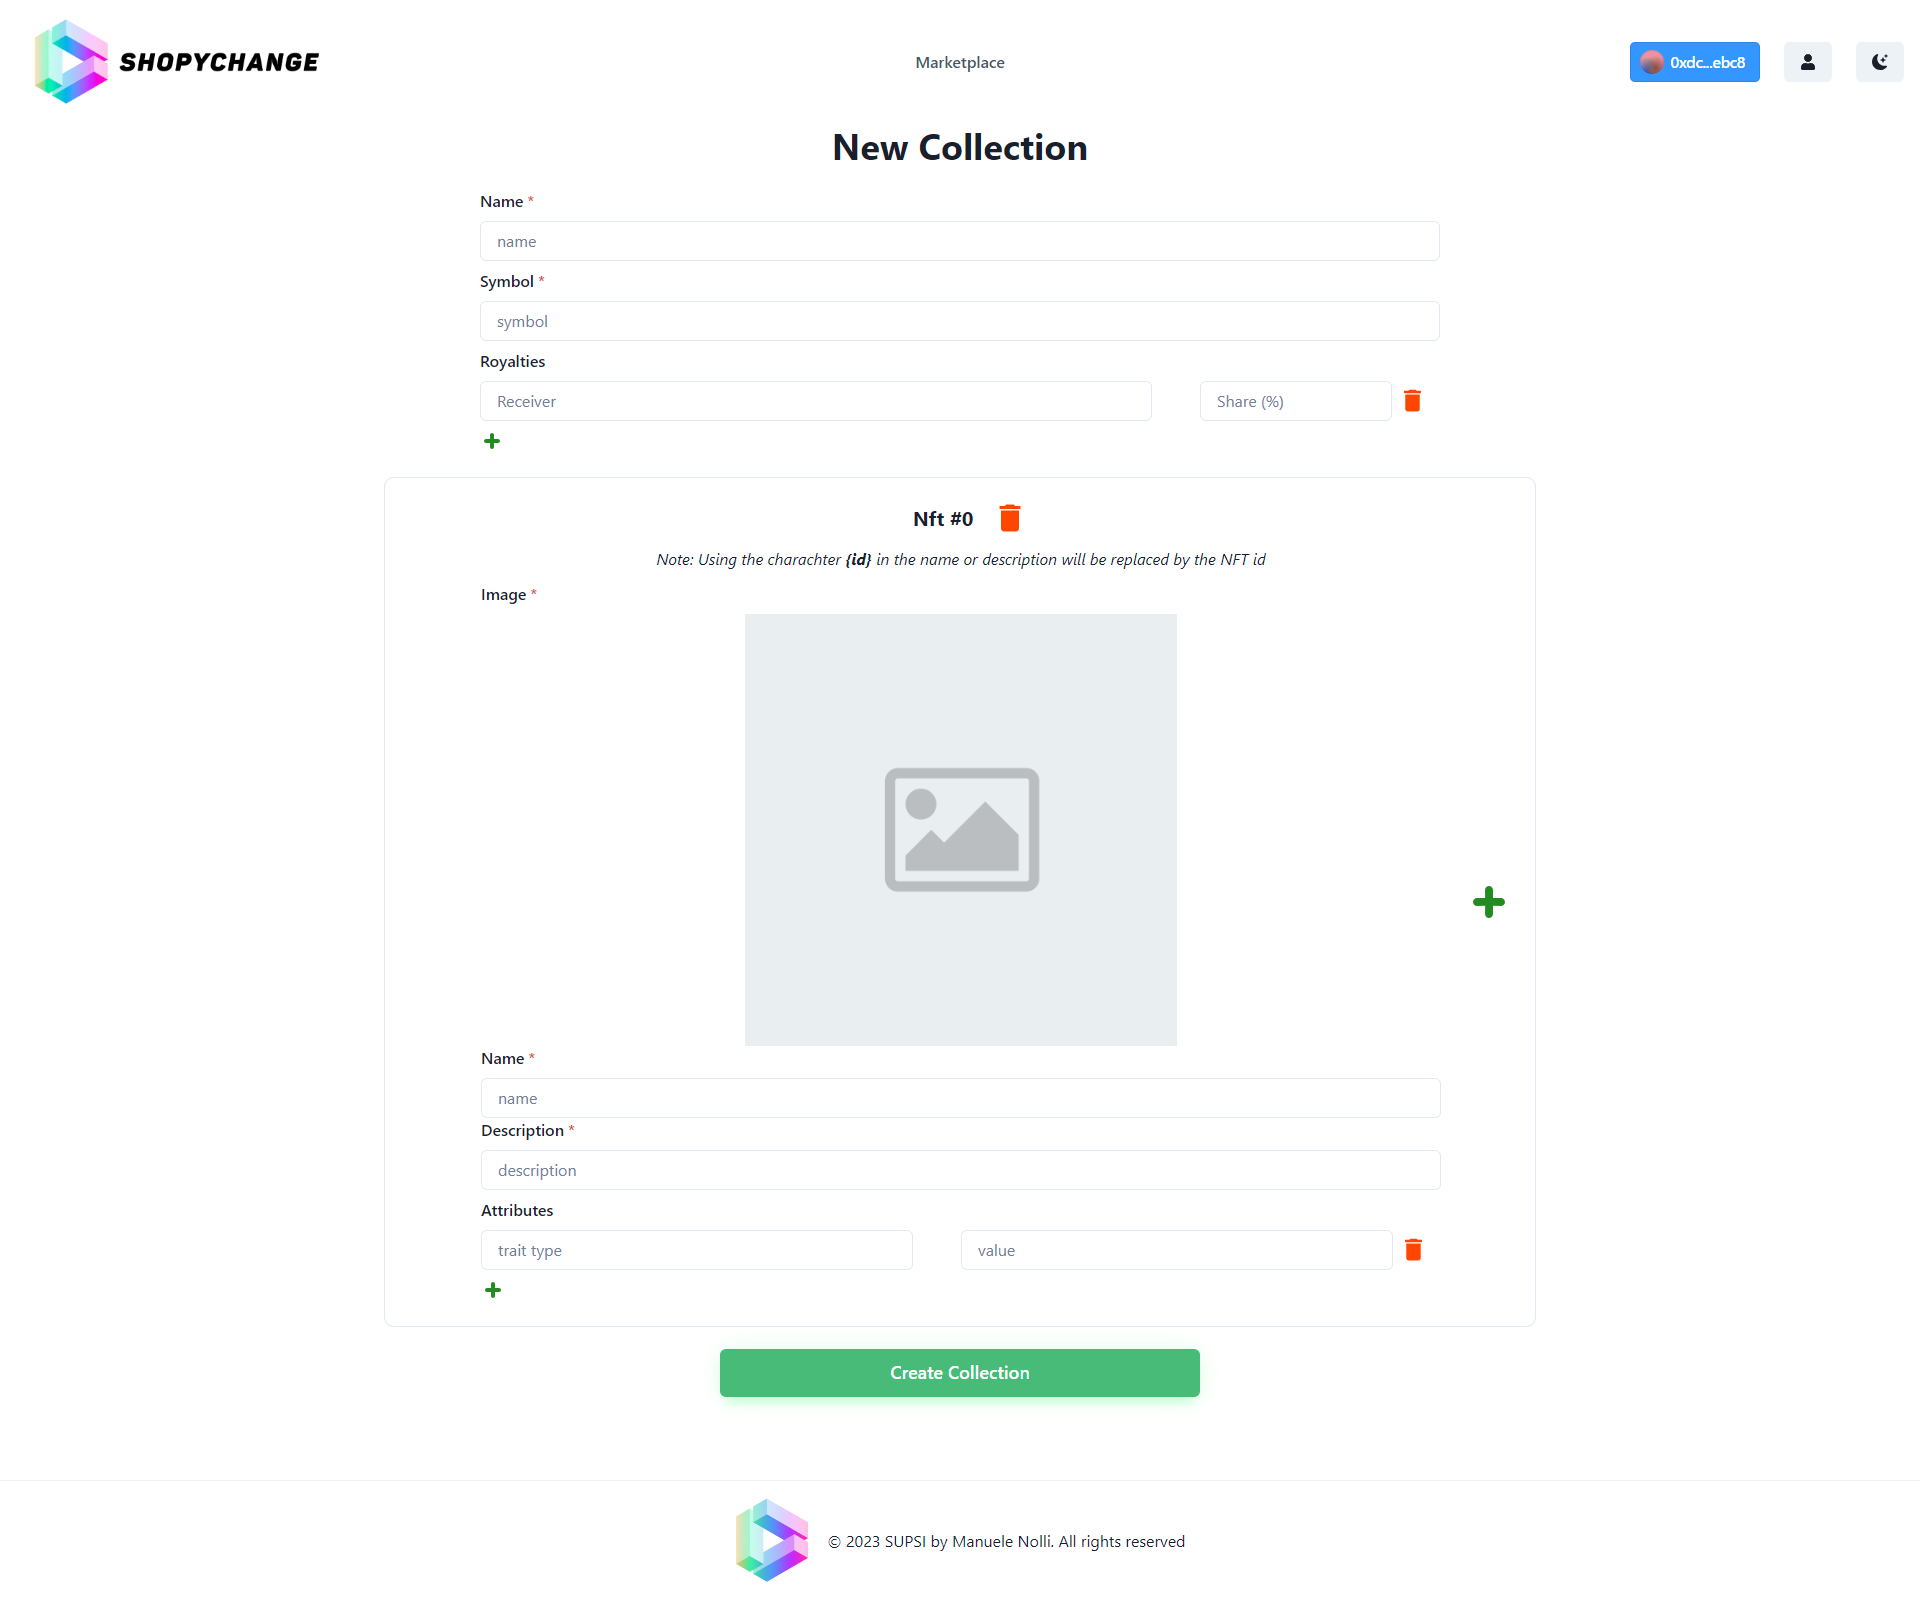
\includegraphics[width=\textwidth]{images/pages/createCollection.png}}
    \end{minipage}
    \hfill
    \begin{minipage}{0.26\textwidth }
      \centering
      \fcolorbox{mint-cream}{white}{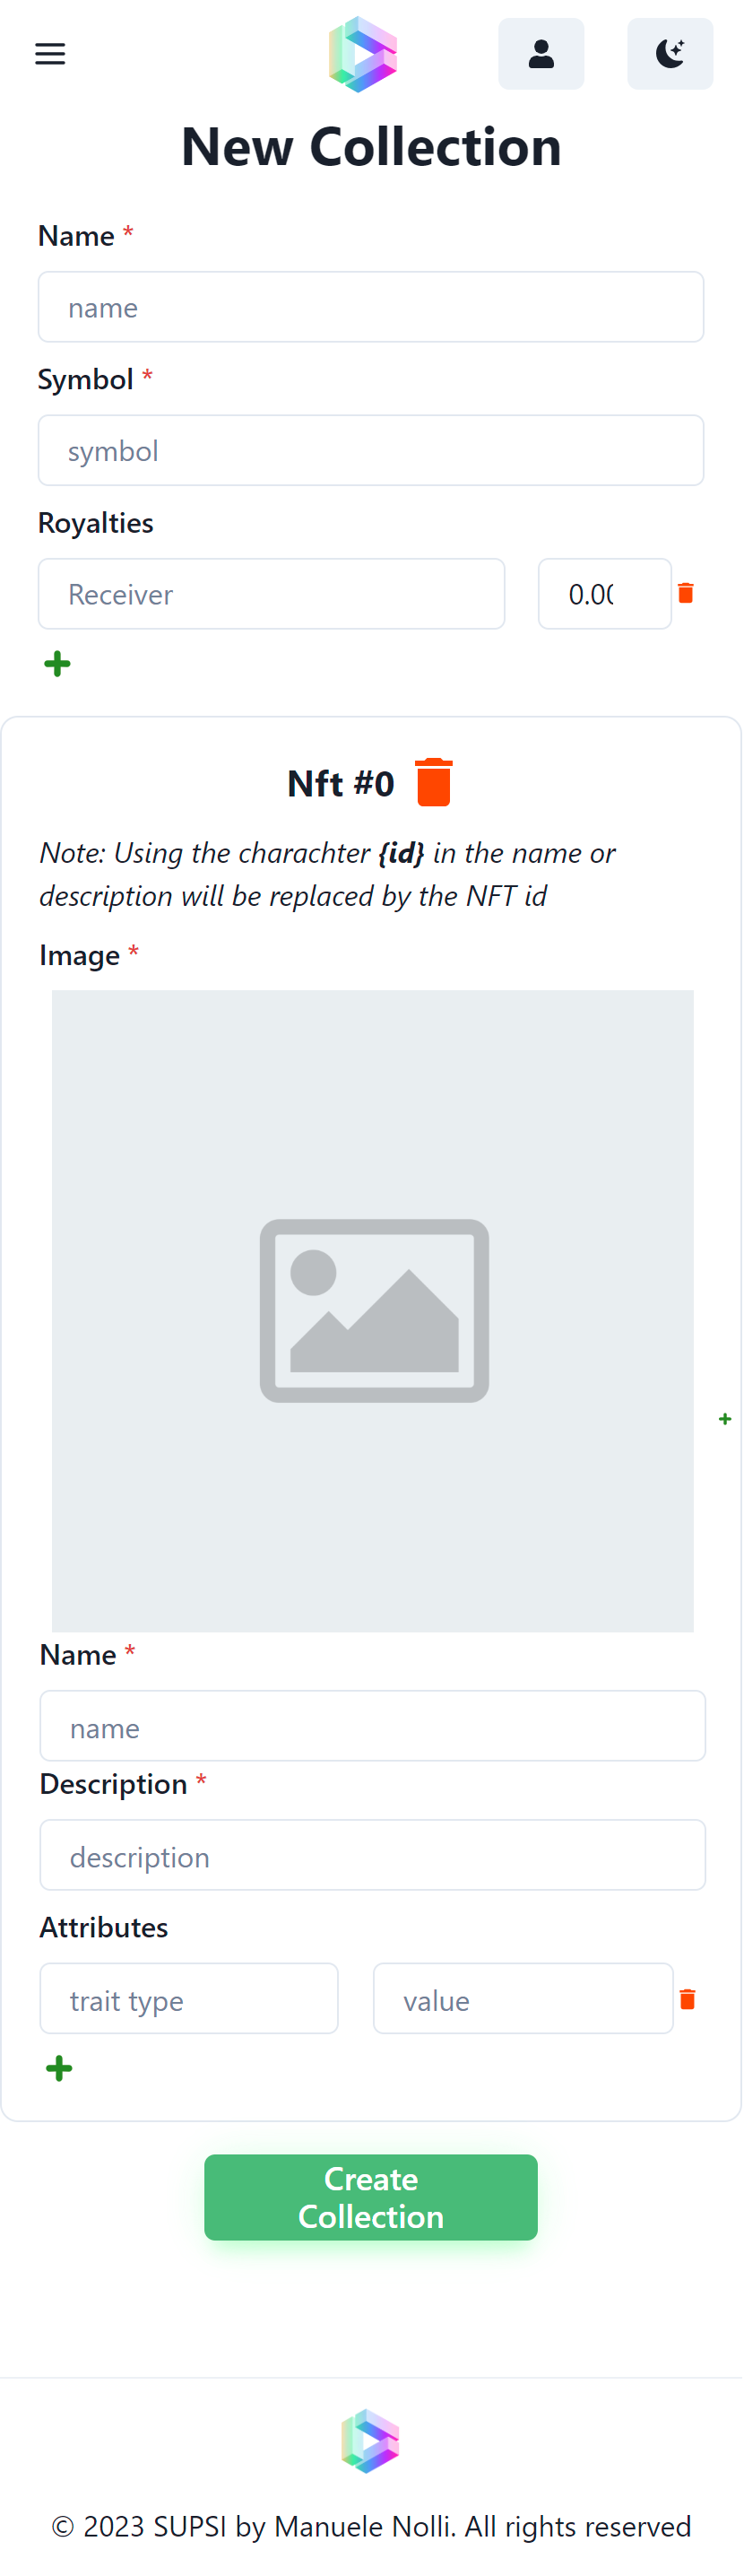
\includegraphics[width=\textwidth]{images/pages/createCollection_mobile.png}}
      \end{minipage}
      \caption{Pagina Creazione collezione}
      \label{fig:create-collection}
  \end{figure}

\subsubsection{Visualizzazione NFT} 

La seguente pagina permette di visualizzare tutte le informazioni riguardo ad un NFT. Ovvero, i dati del contratto, l'attuale possessore, i metadati dell'NFT e la cronologia di spostamento. Inoltre, la pagina cambia aspetto in base all'utente connesso e allo stato dell'NFT. La pagina è visibile con tema scuro in figura \ref{fig:visualizzazione-nft}.

\begin{figure}[H]
    \begin{minipage}{0.7\textwidth}
      \centering
      \fcolorbox{mint-cream}{white}{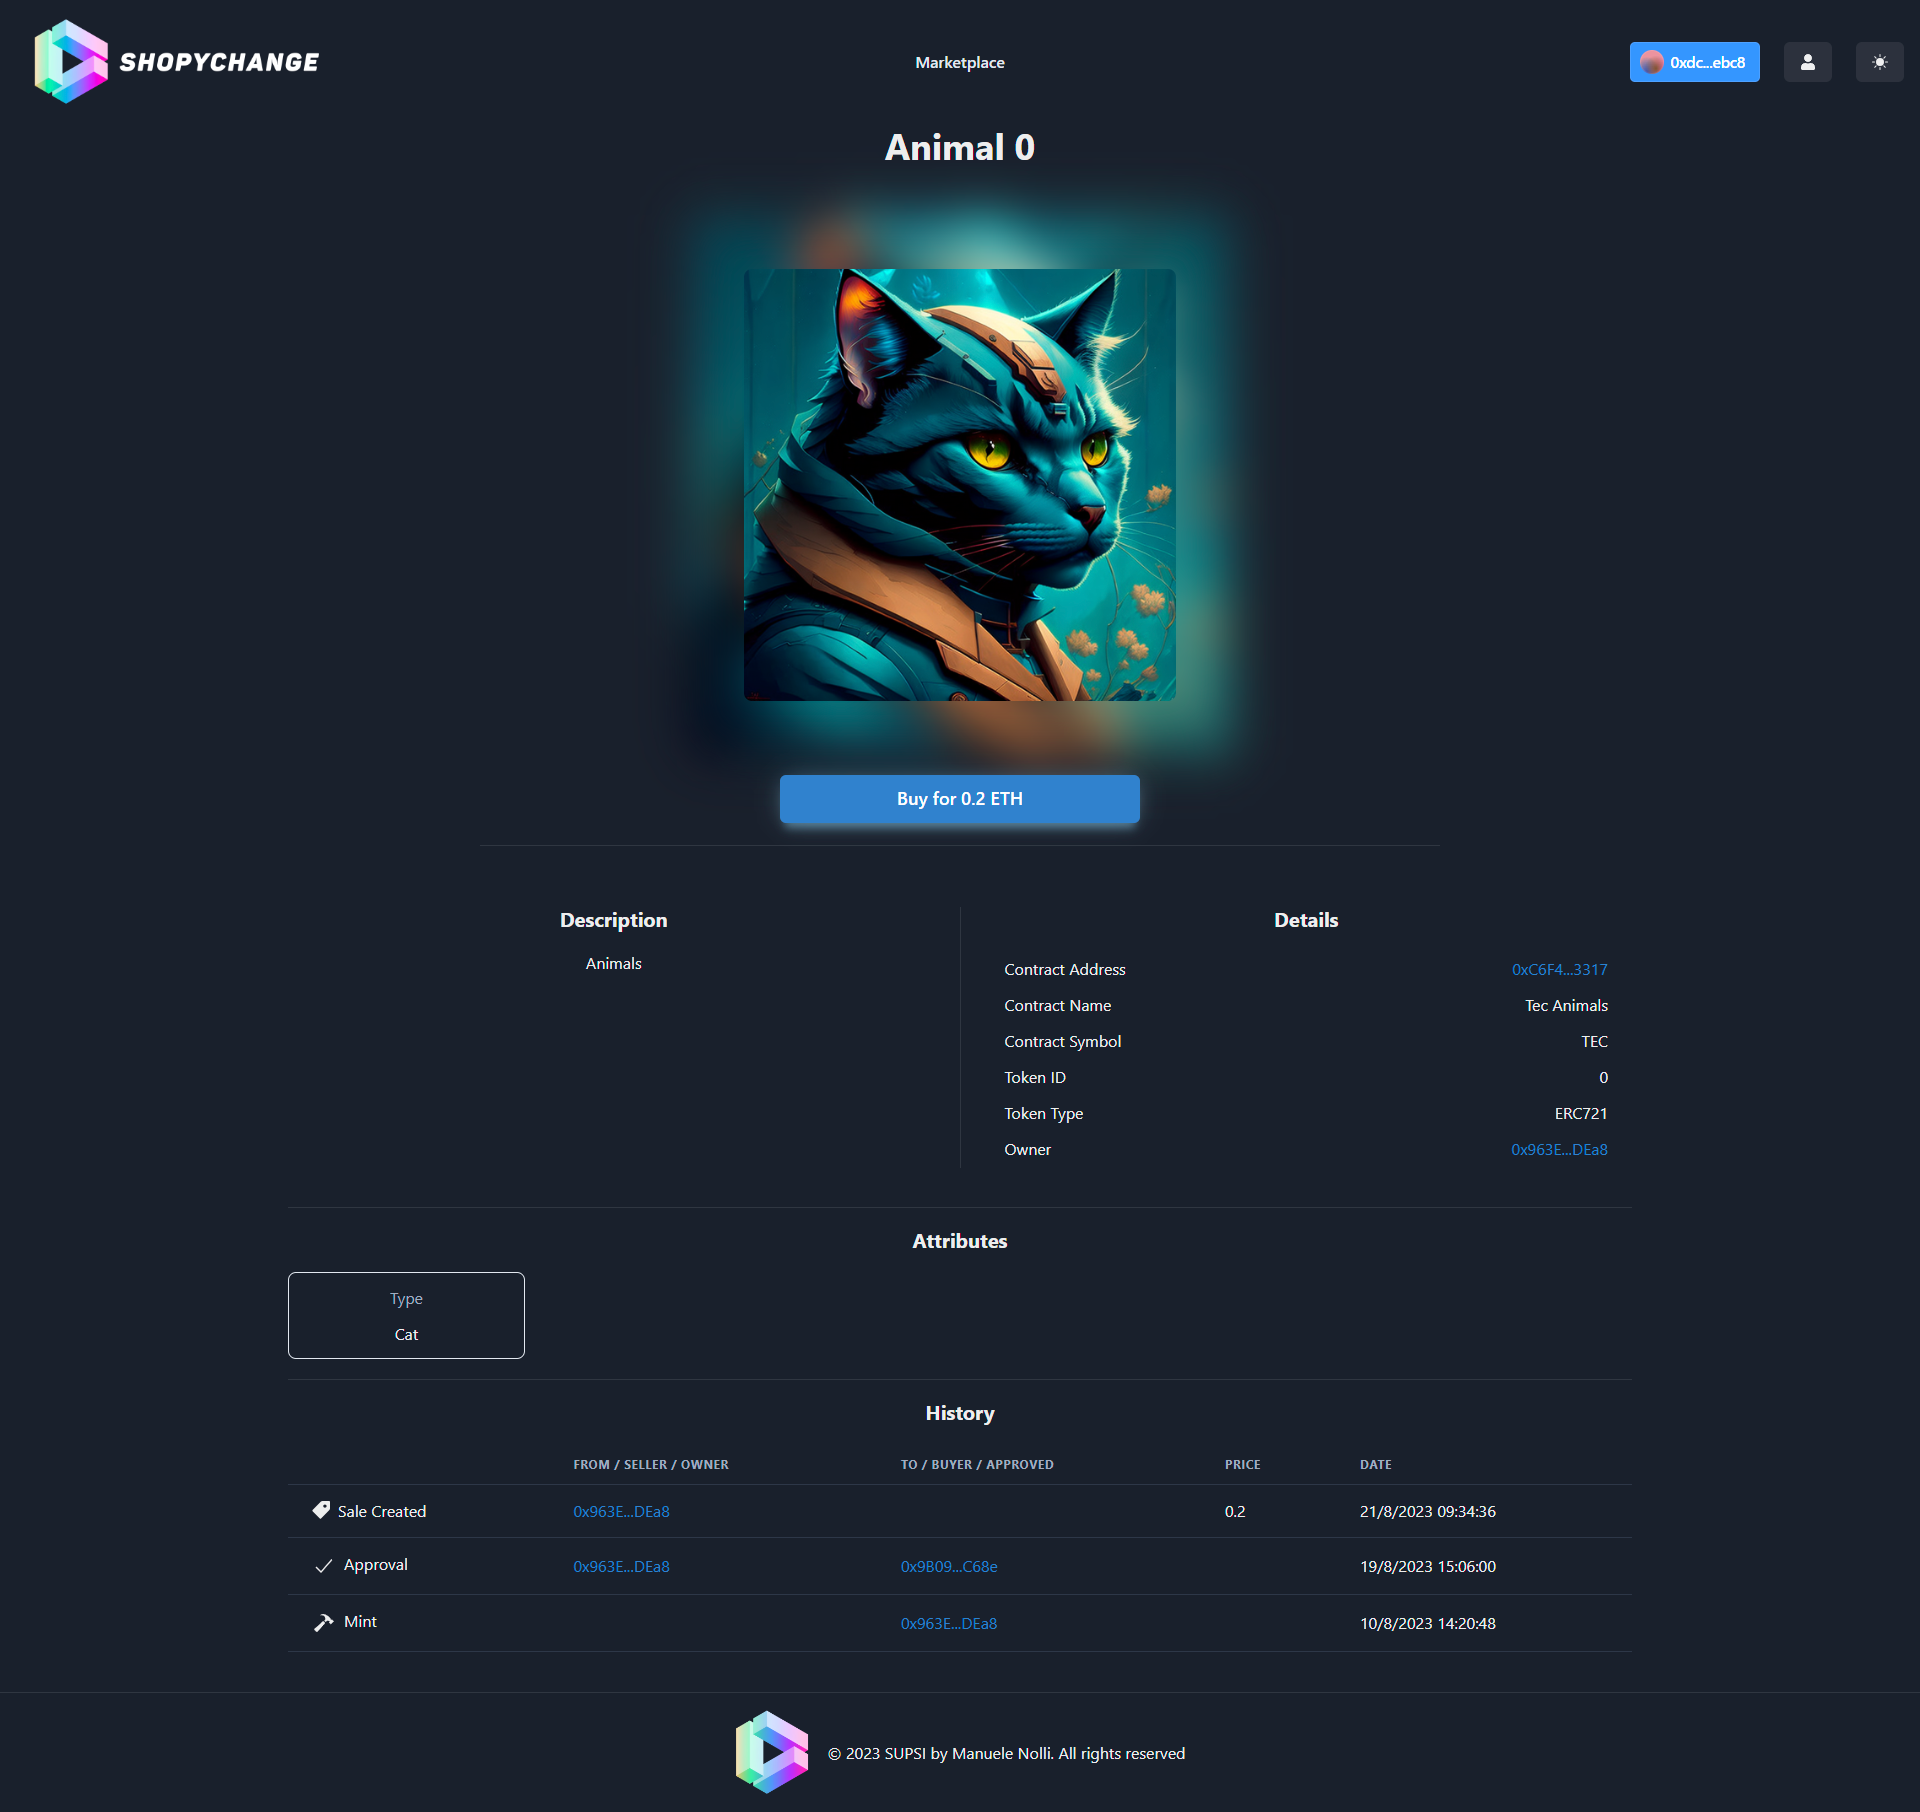
\includegraphics[width=\textwidth]{images/pages/nftPage.png}}
    \end{minipage}
    \hfill
    \begin{minipage}{0.26\textwidth }
      \centering
      \fcolorbox{mint-cream}{white}{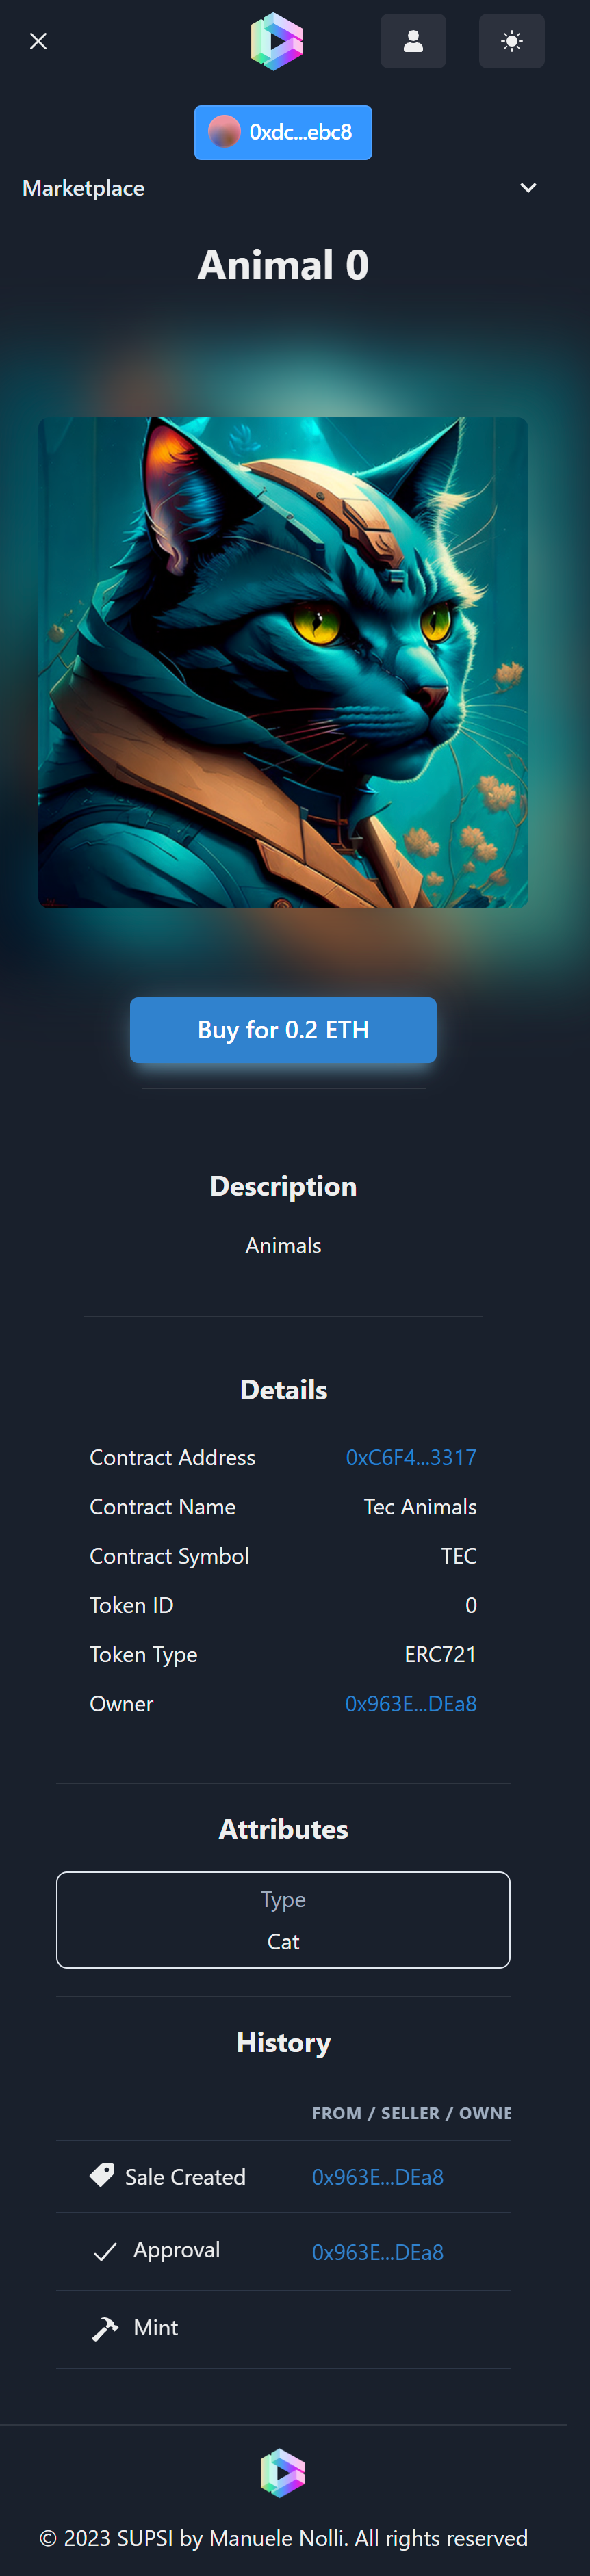
\includegraphics[width=\textwidth]{images/pages/nftPage_mobile.png}}
      \end{minipage}
      \caption{Pagina Visualizzazione NFT}
      \label{fig:visualizzazione-nft}
  \end{figure}

\subsubsection{Vendita, Acquisto, Modifica e Cancellazione}

Le operazione di messa vendita, acquisto, modifica e cancellazione di una vendita sono gestite tramite modali. Perciò, non è presente una pagina dedicata a queste operazioni ma sono presenti in diverse pagine. La figura \ref{fig:modal} mostra un esempio di messa in vendita di un NFT. Come è possibile notare, il modale presenta una tabella con le informazioni riguardanti alla divisione del prezzo di vendita. 

\begin{figure}[H]
    \begin{minipage}{0.7\textwidth}
      \centering
      \fcolorbox{mint-cream}{white}{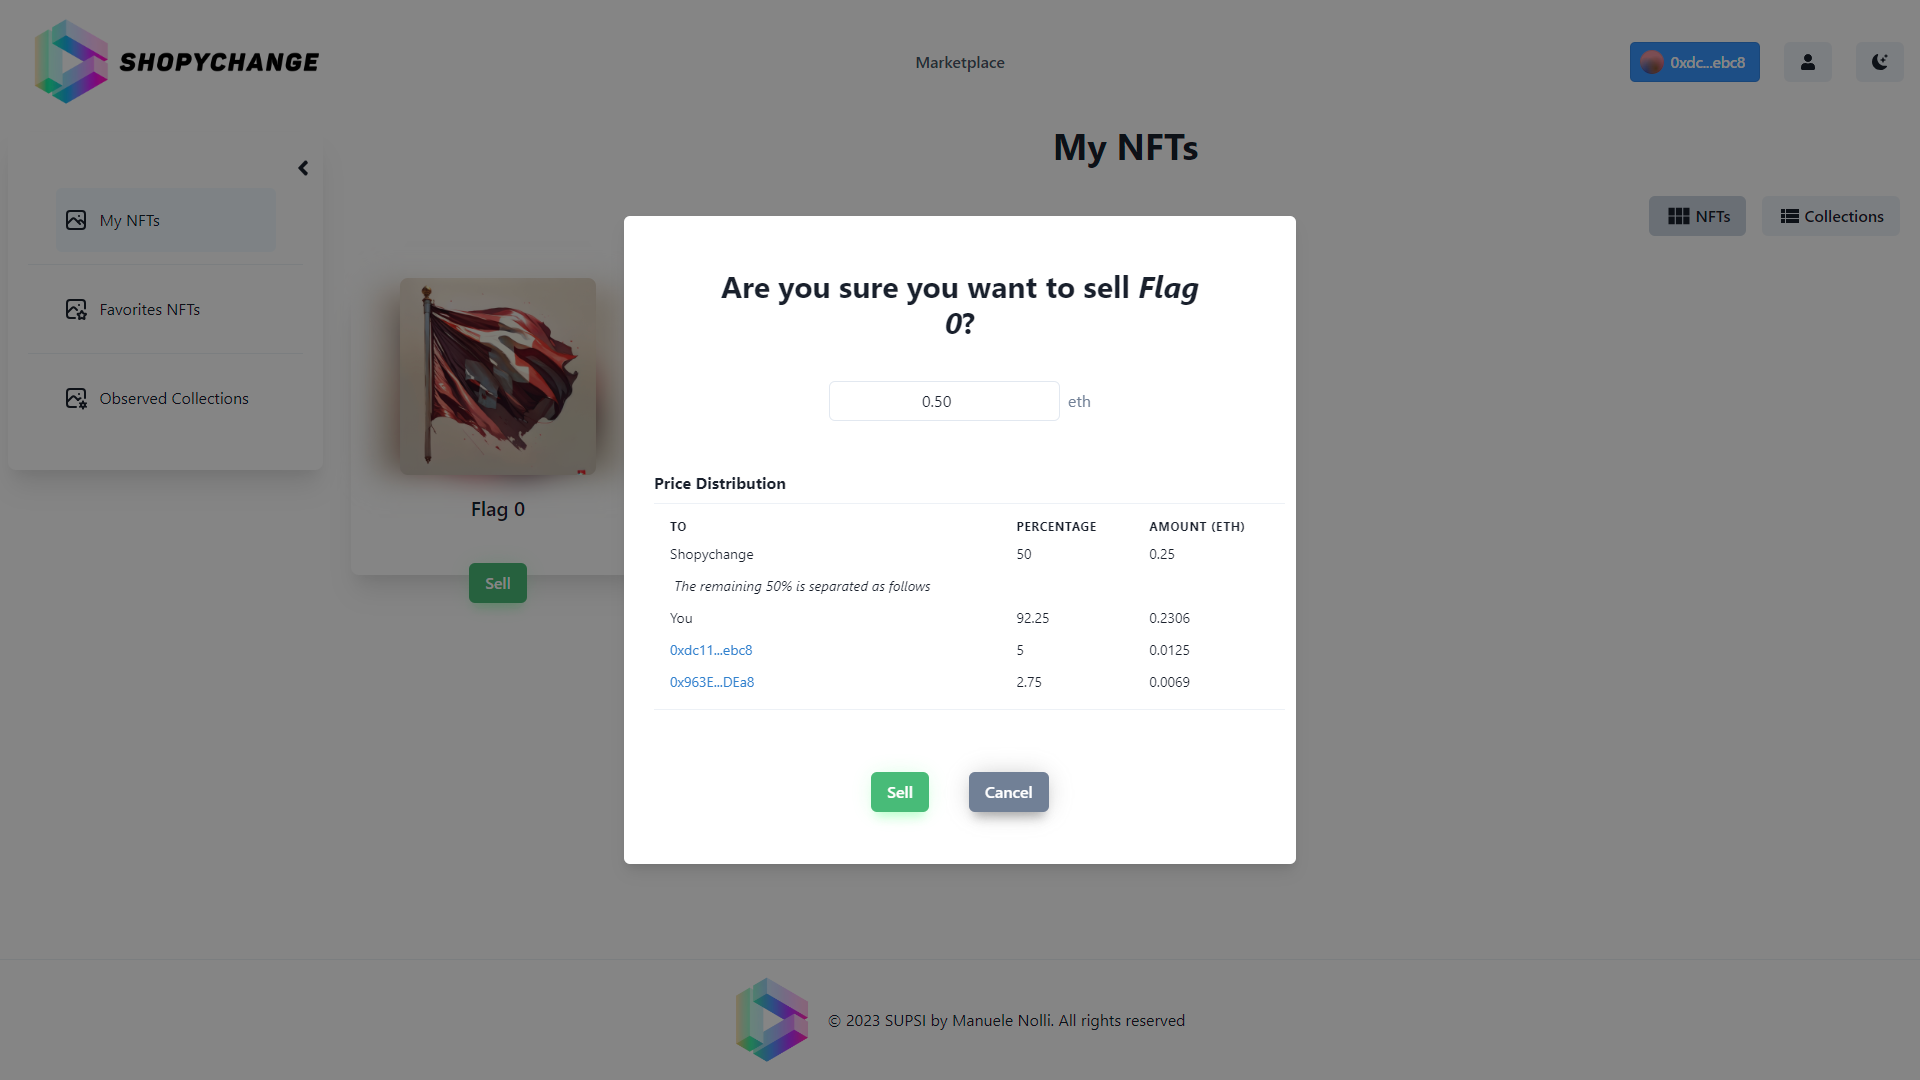
\includegraphics[width=\textwidth]{images/pages/sell.png}}
    \end{minipage}
    \hfill
    \begin{minipage}{0.26\textwidth }
      \centering
      \fcolorbox{mint-cream}{white}{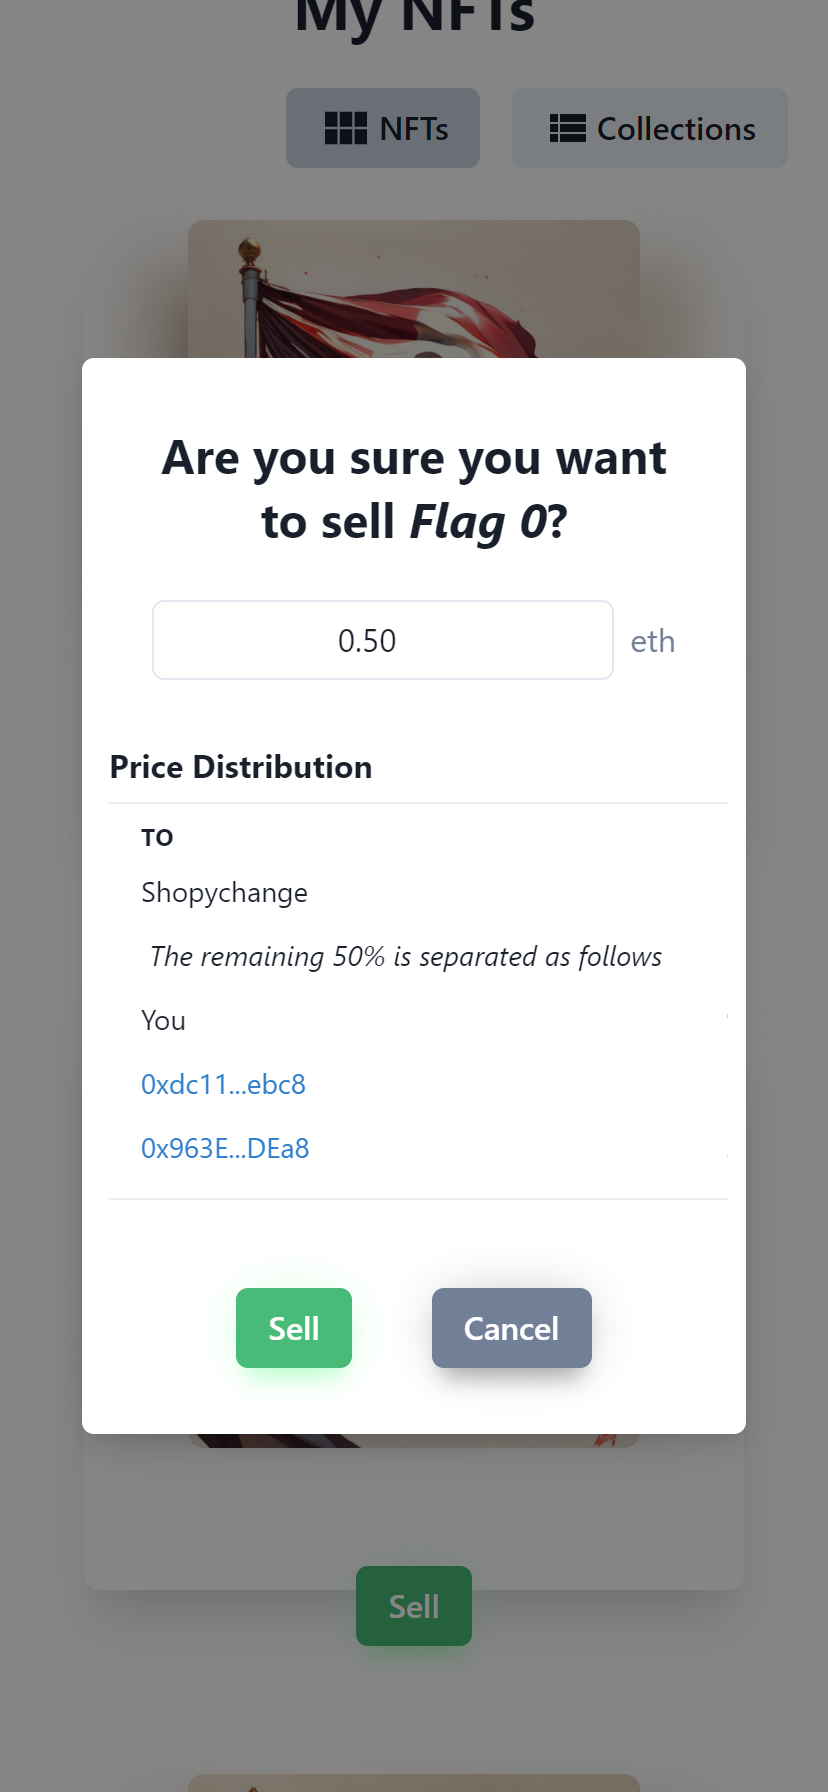
\includegraphics[width=\textwidth]{images/pages/sell_mobile.png}}
      \end{minipage}
      \caption{Modale Acquisto NFT}
      \label{fig:modal}
  \end{figure}

\subsubsection{Modifica Royalty}

  L'applicativo presenta due pagine per la modifica delle royalty. La prima rappresenta la modifica delle royalty di default per la collezione intera. La seconda pagina, visibile in figura \ref{fig:modifica-royalty}, permette di modificare le royalty di un singolo NFT, sganciandosi dalla royalty di default.

  \begin{figure}[H]
    \begin{minipage}{0.7\textwidth}
      \centering
      \fcolorbox{mint-cream}{white}{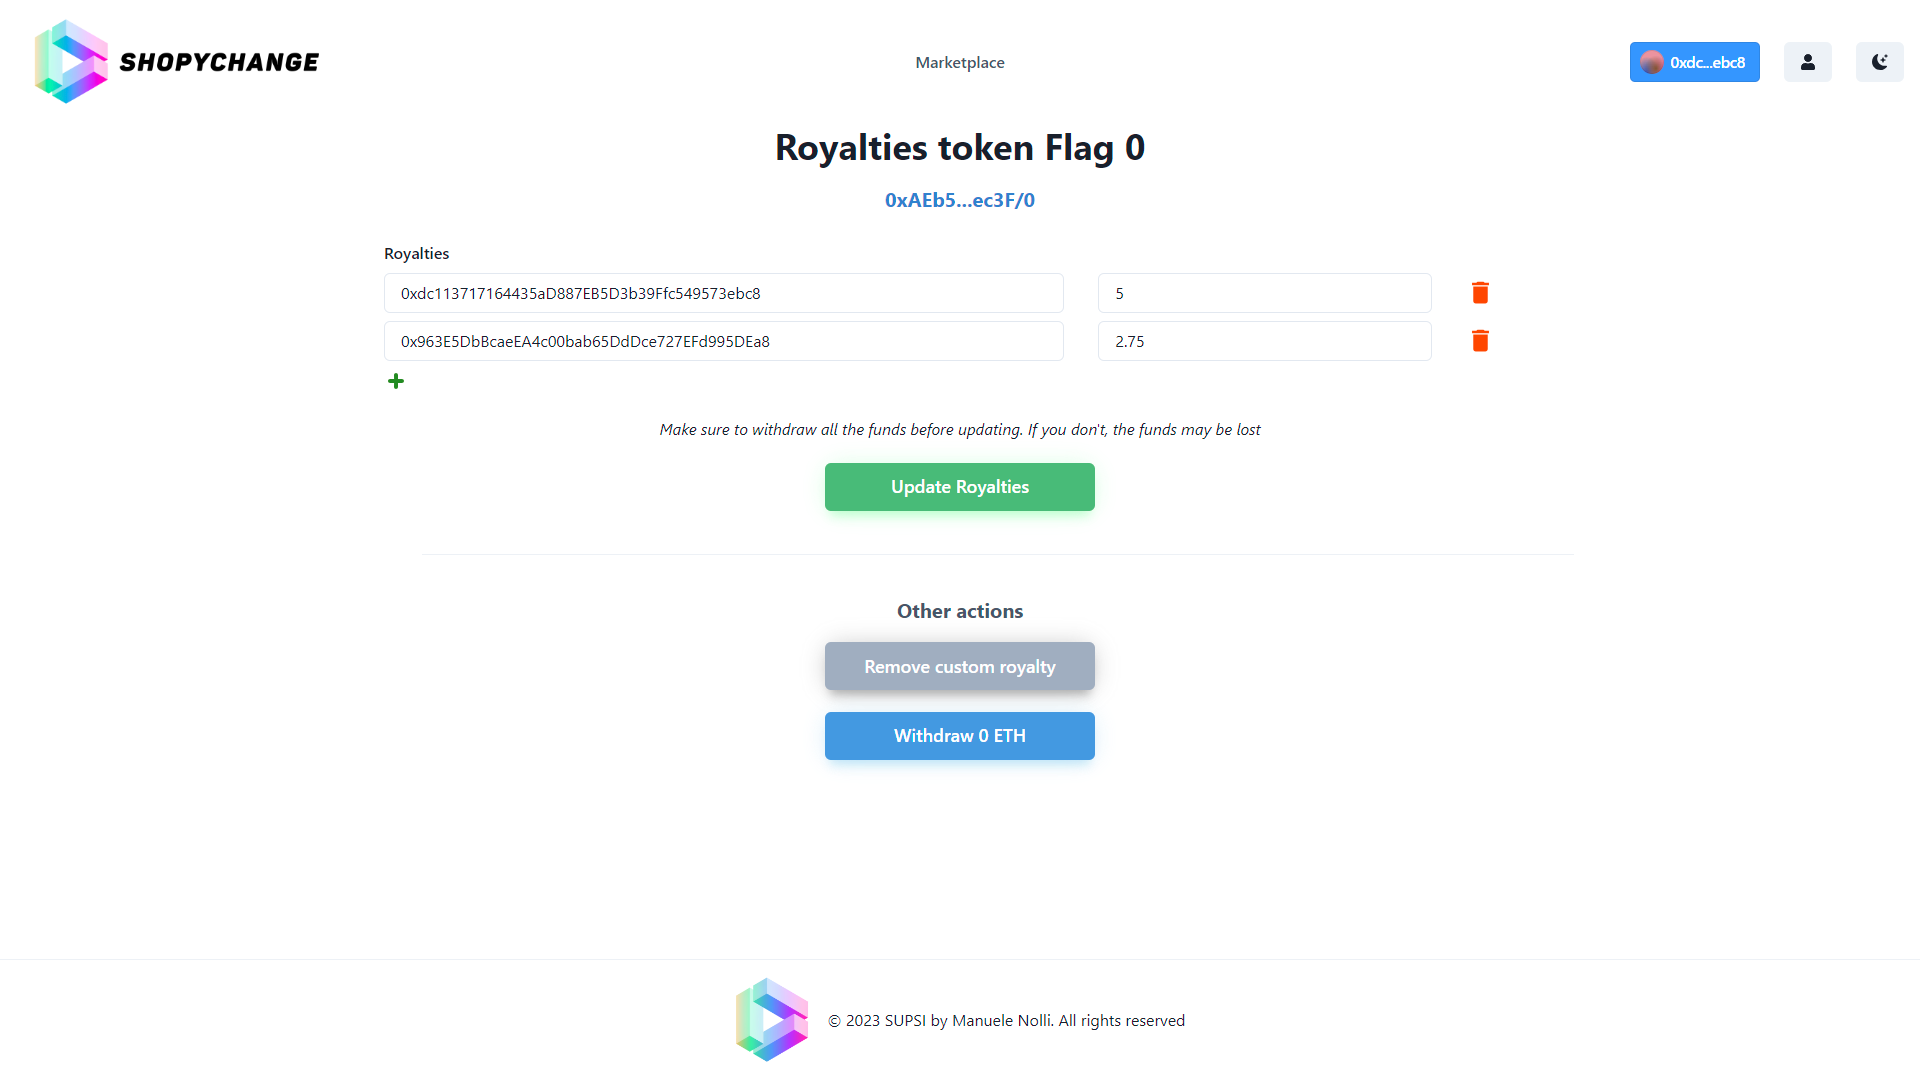
\includegraphics[width=\textwidth]{images/pages/tokenRoyalty.png}}
    \end{minipage}
    \hfill
    \begin{minipage}{0.26\textwidth }
      \centering
      \fcolorbox{mint-cream}{white}{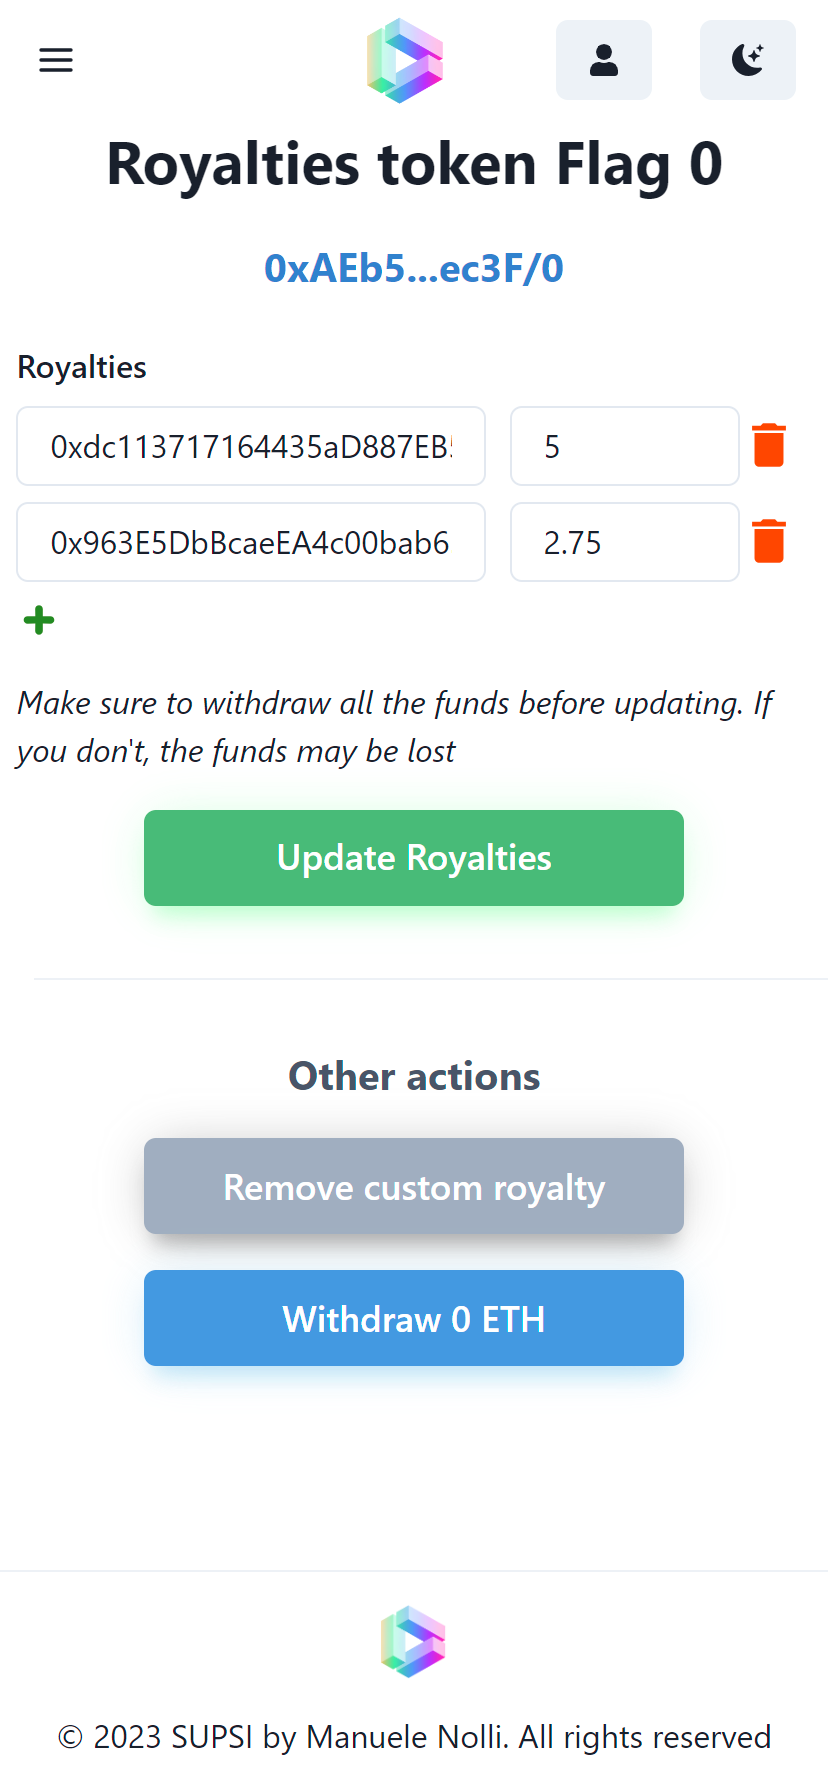
\includegraphics[width=\textwidth]{images/pages/tokenRoyalty_mobile.png}}
      \end{minipage}
      \caption{Pagina Modifica Royalty NFT}
      \label{fig:modifica-royalty}
  \end{figure}

\subsubsection{Admin dashboard}
\label{sec:admin-dashboard}

La pagina \textit{Admin} è raggiungibile unicamente dall'amministratore del marketplace. Al suo interno sono presenti le operazioni per il ritiro e modifica delle royalty a favore del marketplace, oltre a svariate funzionalità di gestione. La pagina è visibile in figura \ref{fig:admin}.

\begin{figure}[H]
    \centering
    \fcolorbox{mint-cream}{white}{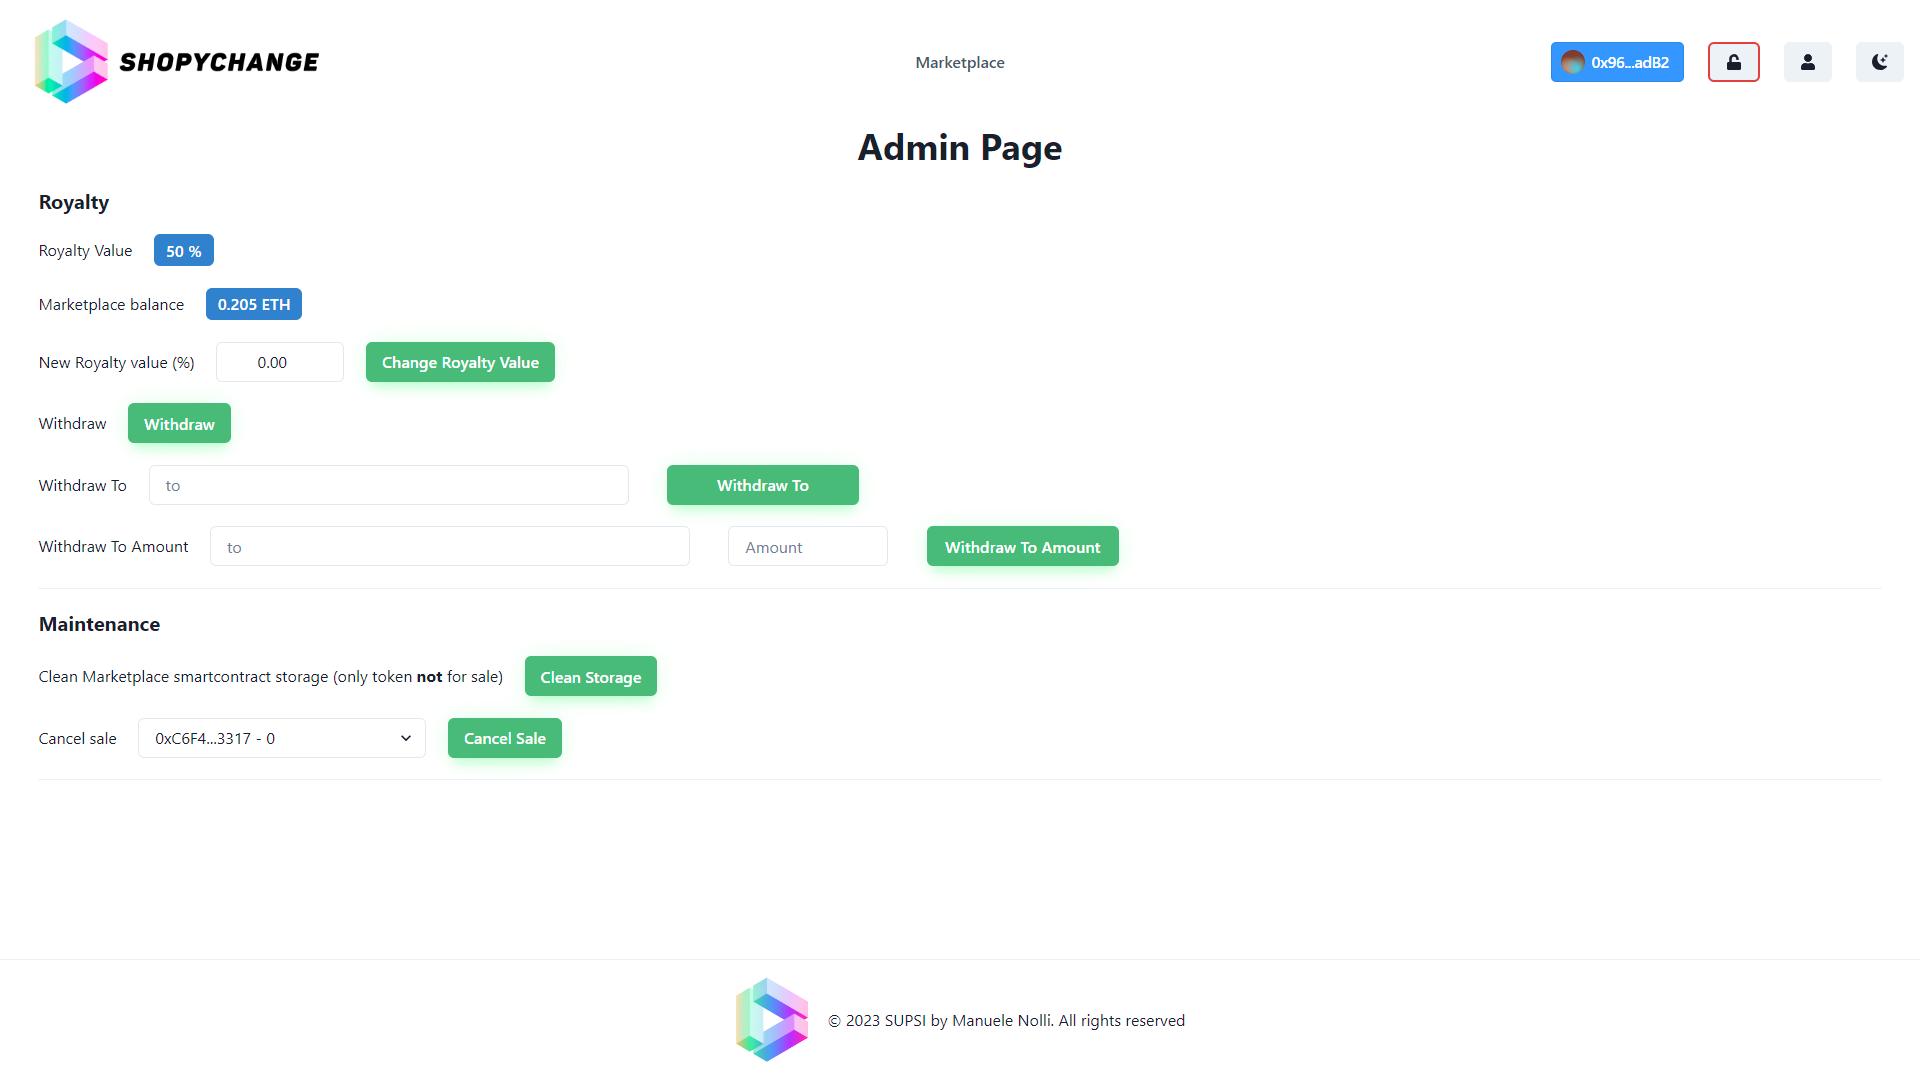
\includegraphics[width=0.8\textwidth]{images/pages/adminPage.png}}
    \caption{Pagina admin}
    \label{fig:admin}
\end{figure}

\subsection{Test}

Grazie all'organizzazione strutturale descritta nei precedenti capitoli ogni operazione è stata testata in modo efficace. I test sono stati scritti grazie all'aiuto della libreria \textit{jest}\footnote{https://jestjs.io/}, la quale permette di creare \textit{unit test}, \textit{snapshot test} e \textit{integration test}. Infatti, i test creati verificano la corretta visualizzazione grafica, il funzionamento in modo indipendente e l'integrazione con altri componenti.

In aggiunta, è stato utilizzato lo strumento \textit{Cypress}\footnote{https://www.cypress.io/} per la creazione di \textit{end-to-end test}. Questi test permettono di simulare l'interazione dell'utente con l'applicazione e di conseguenza di verificare il corretto funzionamento dell'applicativo. \textit{Cypress} è stato utilizzato in combinazione con \textit{Synpress}\footnote{https://github.com/Synthetixio/synpress}, ovvero uno strumento che permette la configurazione del wallet \textit{Metamask} all'interno del browser indipendente di \textit{Cypress}. In questo modo è stato possibile testare anche le funzionalità che richiedono l'interazione con la blockchain. Purtroppo però, a causa dell'impossibilità di verificare il funzionamento del pulstante di \textit{WalletConnect}, che permette la connessione del wallet, non è stato possibile testare le funzionalità che richiedono l'interazione con la blockchain. 

\subsection{Motivazioni e Alternative}

Il requisito per il modulo \textit{frontend} comprendeva l'utilizzo di \textit{Javascript}, ma essendo \textit{Typescript} un superset è stato deciso di utilizzare quest'ultimo in modo da ridurre gli errori di programmazione grazie ai tipi. La scelta del framework è stata fatta in base alla compatibilità delle librerie di comunicazione con la blockchain. Le alternative erano \textit{Angular}\footnote{https://angular.io/} e \textit{Vue}\footnote{https://vuejs.org/} ma la libreria \textit{WalletConnect} è maggiormente compatibile con \textit{React}.
 
La libreria \textit{WalletConnect} è stata scelta per la sua semplicità d'uso e la sua compatibilità con diversi wallet. Inoltre, risulta essere un protocollo più maturo rispetto alla sua alternativa principale, cioè \textit{RainbowKit}\footnote{https://www.rainbowkit.com/} che è attualmente alla versione 1.0.9.

In aggiunta, avendo scelto \textit{WalletConnect} è consigliato utilizzare \textit{Wagmi} invece di \textit{ethers.js} o \textit{web3.js}, in quanto l'integrazione tra \textit{WalletConnect} e \textit{ethers.js} risulta essere più complessa.

Per quanto riguarda la libreria grafica, la scelta è stata personale in quanto esistono diverse alternative valide come \textit{Material UI}\footnote{https://material-ui.com/} e \textit{Ant Design}\footnote{https://ant.design/}. \textit{ChakraUI} è stata scelta per la completezza e grafica dei componenti.